%%%%%%%%%%%%%%%%%%%%%%%%%%%%%%%%%%%%%%%%%
% Journal Article
% LaTeX Template
% Version 1.3 (9/9/13)
%
% This template has been downloaded from:
% http://www.LaTeXTemplates.com
%
% Original author:
% Frits Wenneker (http://www.howtotex.com)
%
% License:
% CC BY-NC-SA 3.0 (http://creativecommons.org/licenses/by-nc-sa/3.0/)
%
%%%%%%%%%%%%%%%%%%%%%%%%%%%%%%%%%%%%%%%%%

%----------------------------------------------------------------------------------------
%	PACKAGES AND OTHER DOCUMENT CONFIGURATIONS
%----------------------------------------------------------------------------------------

\documentclass[twoside]{article}


\usepackage{lipsum} % Package to generate dummy text throughout this template
\usepackage[sc]{mathpazo} % Use the Palatino font
\usepackage[T1]{fontenc} % Use 8-bit encoding that has 256 glyphs
\linespread{1.05} % Line spacing - Palatino needs more space between lines
\usepackage{microtype} % Slightly tweak font spacing for aesthetics

\usepackage[hmarginratio=1:1,top=32mm,columnsep=20pt]{geometry} % Document margins
\usepackage{multicol} % Used for the two-column layout of the document
\usepackage[hang, small,labelfont=bf,up,textfont=it,up]{caption} % Custom captions under/above floats in tables or figures
\usepackage{booktabs} % Horizontal rules in tables
\usepackage{float} % Required for tables and figures in the multi-column environment - they need to be placed in specific locations with the [H] (e.g. \begin{table}[H])
\usepackage{hyperref} % For hyperlinks in the PDF

\usepackage{graphicx}

\usepackage{lettrine} % The lettrine is the first enlarged letter at the beginning of the text
\usepackage{paralist} % Used for the compactitem environment which makes bullet points with less space between them

\usepackage{abstract} % Allows abstract customization
\renewcommand{\abstractnamefont}{\normalfont\bfseries} % Set the "Abstract" text to bold
\renewcommand{\abstracttextfont}{\normalfont\small\itshape} % Set the abstract itself to small italic text

\usepackage{titlesec} % Allows customization of titles
\renewcommand\thesection{\Roman{section}} % Roman numerals for the sections
\renewcommand\thesubsection{\Roman{subsection}} % Roman numerals for subsections
\titleformat{\section}[block]{\large\scshape\centering}{\thesection.}{1em}{} % Change the look of the section titles
\titleformat{\subsection}[block]{\large}{\thesubsection.}{1em}{} % Change the look of the section titles

\usepackage{fancyhdr} % Headers and footers
\pagestyle{fancy} % All pages have headers and footers
\fancyhead{} % Blank out the default header
\fancyfoot{} % Blank out the default footer
\fancyhead[C]{Vaccinating Health Professionals Prior to Patients $\bullet$ April 2021 $\bullet$ Vol. I, No. 1} % Custom header text
\fancyfoot[RO,LE]{\thepage} % Custom footer text


%----------------------------------------------------------------------------------------
%	TITLE SECTION
%----------------------------------------------------------------------------------------

\title{\vspace{-15mm}\fontsize{24pt}{10pt}\selectfont\textbf{The Effect of COVID-19 Vaccinating Health Professionals Prior to Patients }} % Article title

\author{
\large
\textsc{Jacob H, Lauren H, Ethan R, David W}\thanks{A thank you or further information}\\[2mm] % Your name
%\normalsize University of California \\ % Your institution
%\normalsize \href{mailto:john@smith.com}{john@smith.com} % Your email address
\vspace{-5mm}
}
\date{}

%----------------------------------------------------------------------------------------

\begin{document}

\maketitle % Insert title

\thispagestyle{fancy} % All pages have headers and footers

%----------------------------------------------------------------------------------------
%	ABSTRACT
%----------------------------------------------------------------------------------------

\begin{abstract}

\noindent \lipsum[1] % Dummy abstract text

\end{abstract}

%----------------------------------------------------------------------------------------
%	ARTICLE CONTENTS
%----------------------------------------------------------------------------------------

\begin{multicols}{2} % Two-column layout throughout the main article text

\section{Introduction}

\lettrine[nindent=0em,lines=3]{L} orem ipsum dolor sit amet, consectetur adipiscing elit.
\lipsum[2-3] % Dummy text

%------------------------------------------------

\section{Methods}

\subsection{Model Methods}
General process of how the guys created the model. What they chose as parameters, why they chose specific set-up/ structure etc. 
\begin{compactitem}
\item software used
\item Thought process, planning
\item architecture of model chosen and why 
\item how/why parameters were chosen 
\item optimization methods
\item 1-D model set up
\item 2-D model set up
\end{compactitem}

\subsection{Data Analysis Methods}
Process and methods used to gather and then analyze the data. How we ruled out factors, how we ruled in factors, process of elimination etc. 
\begin{compactitem}
	\item Where is data from
	\item How we got it
	\item Pipeline analysis set-up
	\item types of plots generated
	\item Analysis after plots-- how we determined "significance" in event analysis
	\item What constitutes ruling in a parameter; ruling out a parameter 
	\item What constitutes a likely conclusion
\end{compactitem}
%------------------------------------------------

\section{Results}
\subsection{Model Results}
\rule{\linewidth}{0.25pt}

\subsubsection{Jake's Model Results}

\subsubsection{Ethan's Model Results}

\subsection{Data Analysis Results}
\rule{\linewidth}{0.25pt}

\subsubsection{National-Level Data Analysis Results}

\begin{figure}[H]
	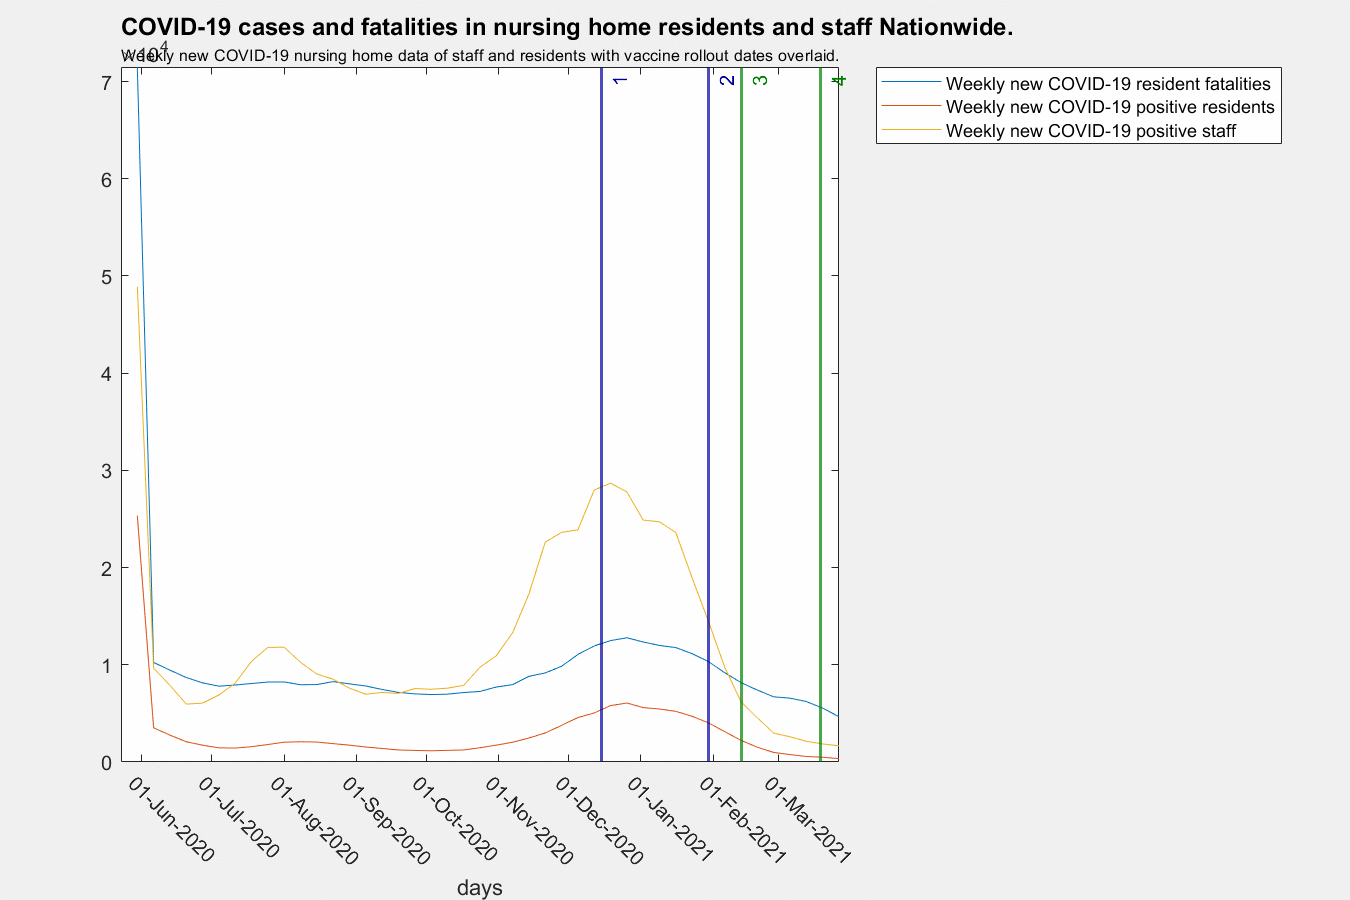
\includegraphics[width=\linewidth]{images/nationwide_nursing_home_with_vaccine.png}
	\caption{The distribution of the first COVID-19 vaccine immediately reduced new COVID-19 cases in nursing home staff Nationwide, followed by a similar reduction in nursing home residents approximately 2 weeks later.  }
	\label{fig:images/nationwide_nursing_home_with_vaccineLabel}
\end{figure}

\subsubsection{State-Level Data Analysis Results}

\begin{figure}[H]
	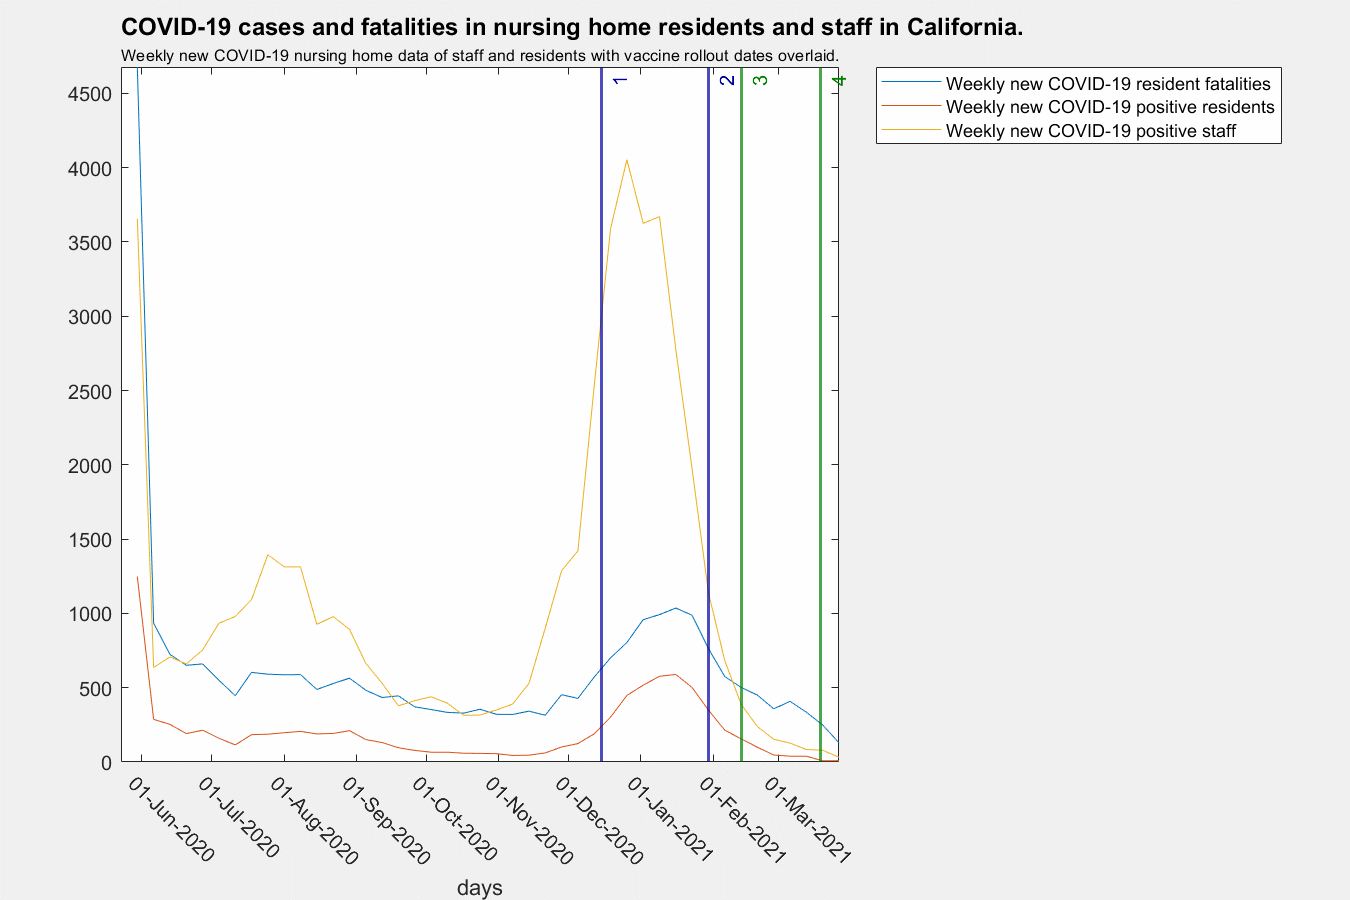
\includegraphics[width=\linewidth]{images/california_nursing_home_with_vaccine.png}
	\caption{Roughly 2 weeks after release of the first COVID-19 vaccine, new COVID-19 cases in nursing home staff in California begins to decline, followed by a reduction in COVID-19 cases and fatalities in residents approximately 2 weeks later. }
	\label{fig:images/california_nursing_home_with_vaccineLabel}
\end{figure}

\begin{figure}[H]
	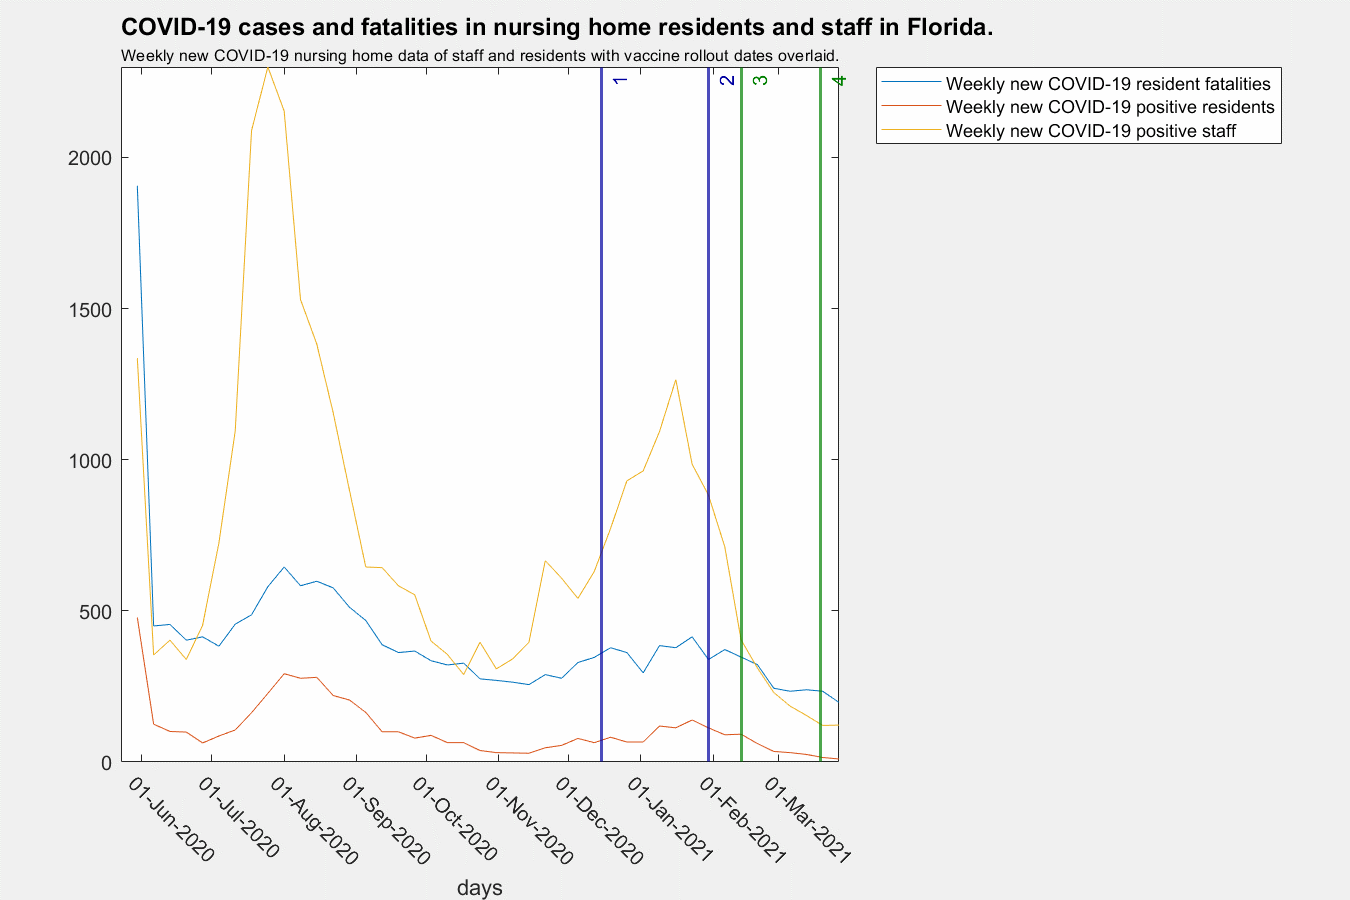
\includegraphics[width=\linewidth]{images/florida_nursing_home_with_vaccine.png}
	\caption{Approximately 4 weeks after the distribution of the first COVID-19 vaccine, new COVID-19 cases in nursing home staff in Florida begin to decline, and COVID-19 cases and fatalities in nursing home residents remained constant for nearly 3 months after the first wave of vaccine distributions before declining.}
	\label{fig:images/florida_nursing_home_with_vaccineLabel}
\end{figure}

\begin{figure}[H]
	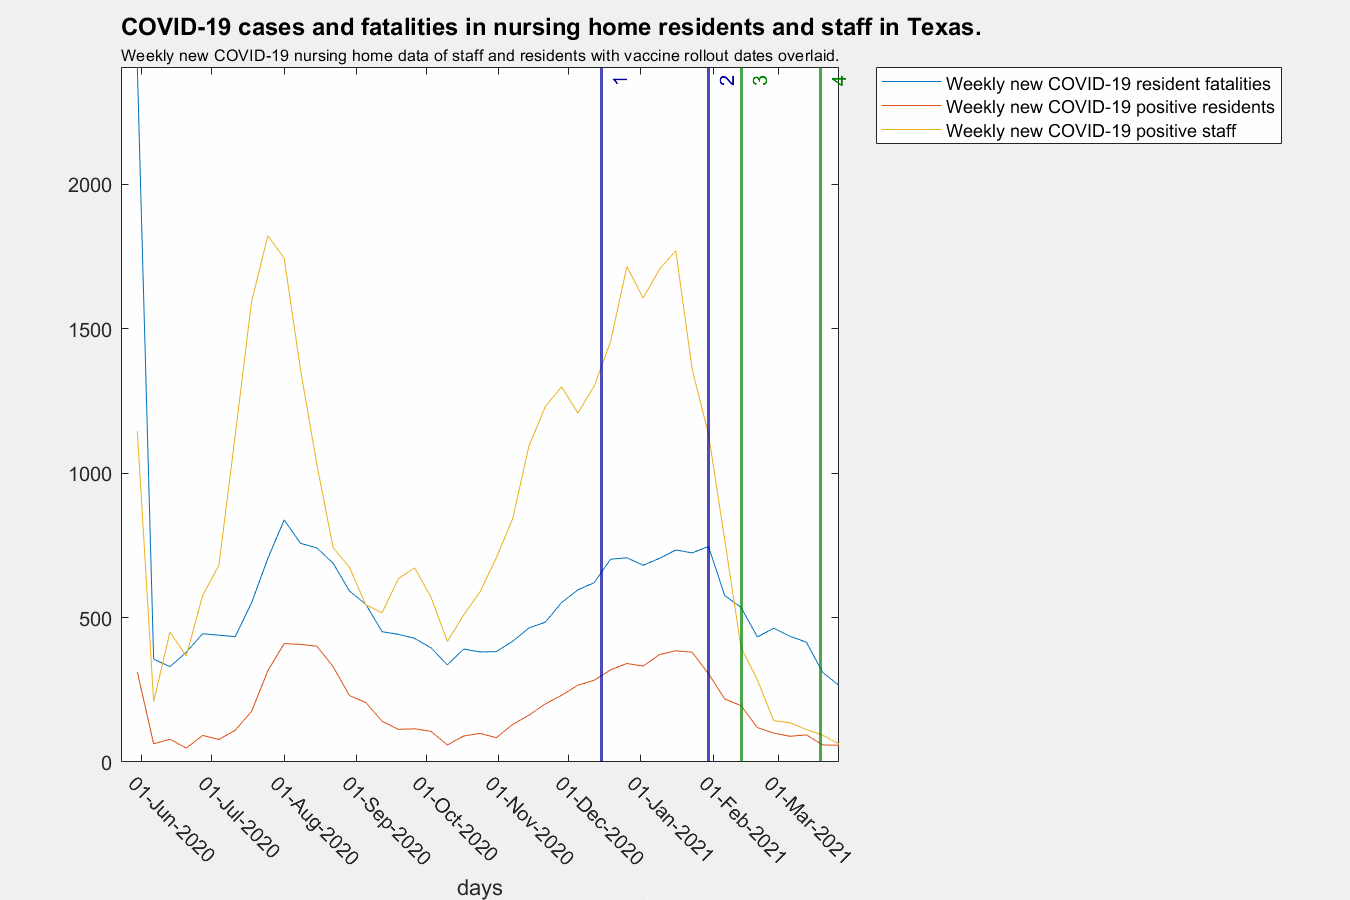
\includegraphics[width=\linewidth]{images/texas_nursing_home_with_vaccine.png}
	\caption{Approximately 4 weeks after the release of the first COVID-19 vaccine, new COVID-19 cases in nursing home staff in Texas began to decline, followed by a decline in COVID-19 cases and fatalities in nursing home residents approximately 1 week later. }
	\label{fig:images/texas_nursing_home_with_vaccineLabel}
\end{figure}

\subsubsection{County-Level Data Analysis Results}

\begin{figure}[H]
	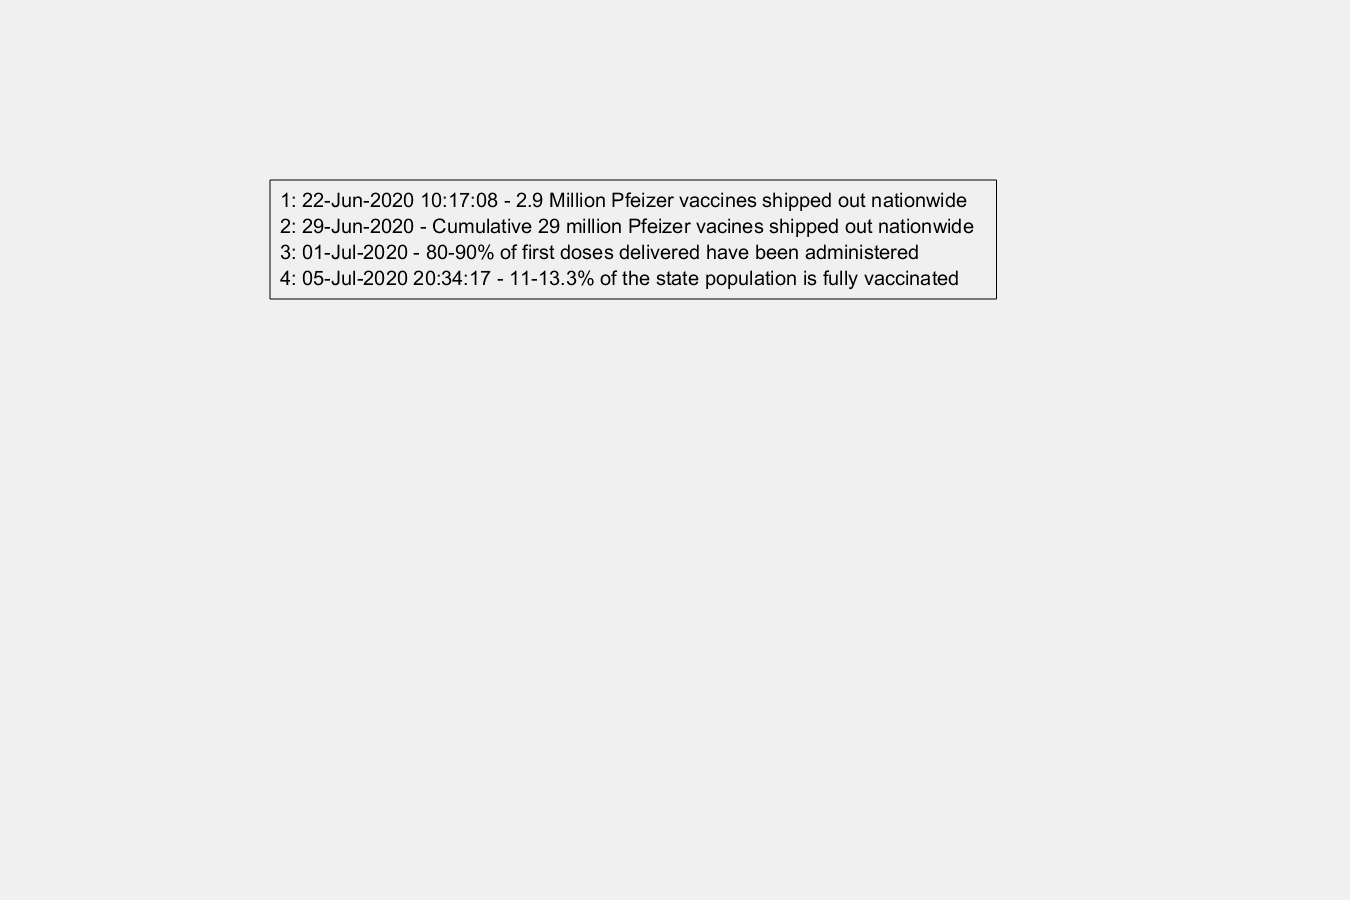
\includegraphics[width=\linewidth]{legends/new_vaccine_rollout_legend.png}
	\caption{}
	\label{fig:legends/new_vaccine_rollout_legendLabel}
\end{figure}


\begin{figure}[H]
	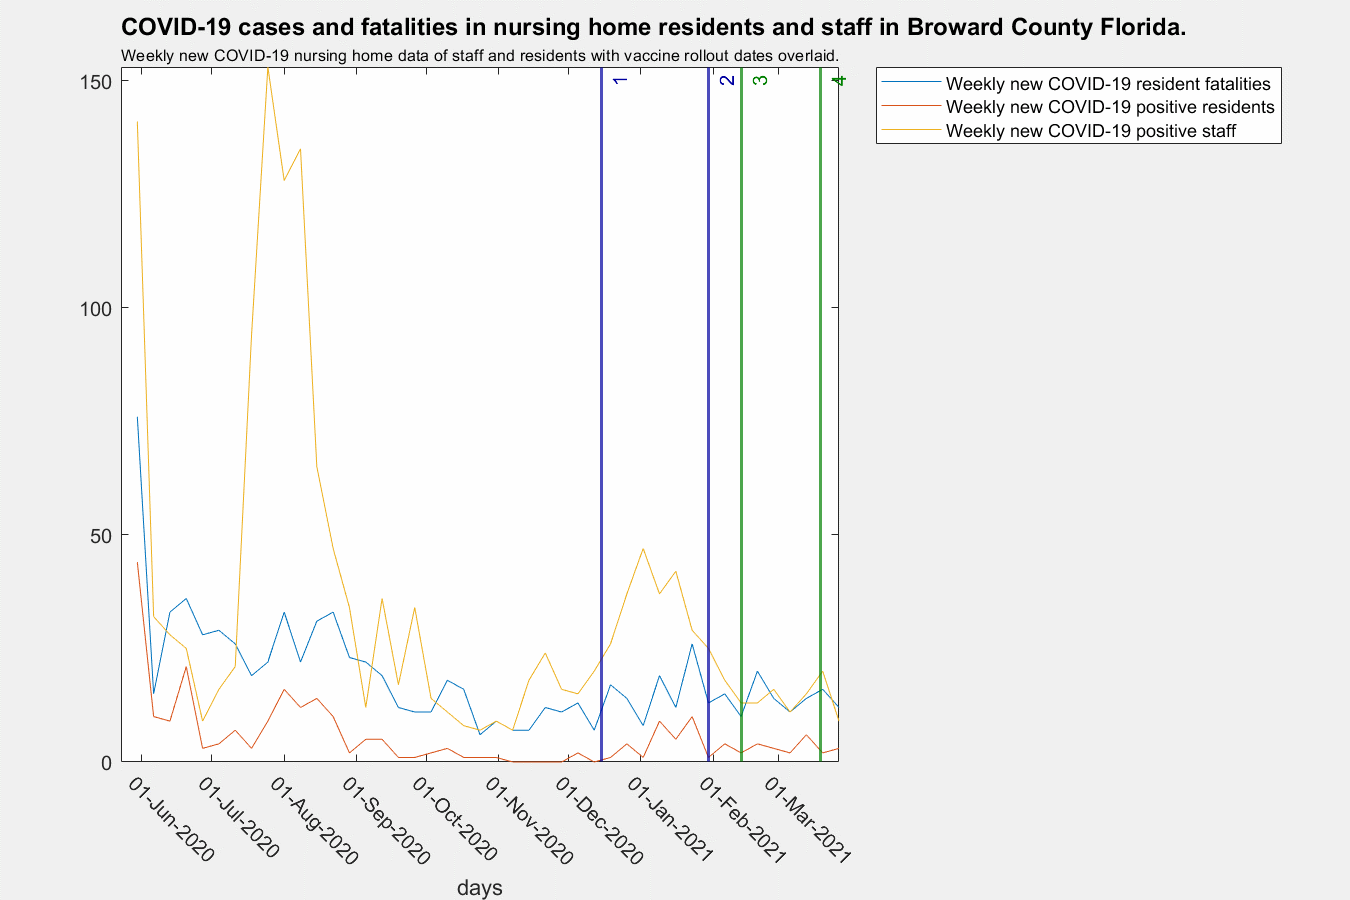
\includegraphics[width=\linewidth]{images/broward_nursing_home_with_vaccine.png}
	\caption{Approximately 2 weeks after COVID-19 vaccine distribution begins, new COVID-19 cases in nursing home staff begin to decline in Broward County Florida,while COVID-19 cases and fatalities in nursing home residents remain constant, displaying no change. }
	\label{fig:images/broward_nursing_home_with_vaccineLabel}
\end{figure}

\begin{figure}[H]
	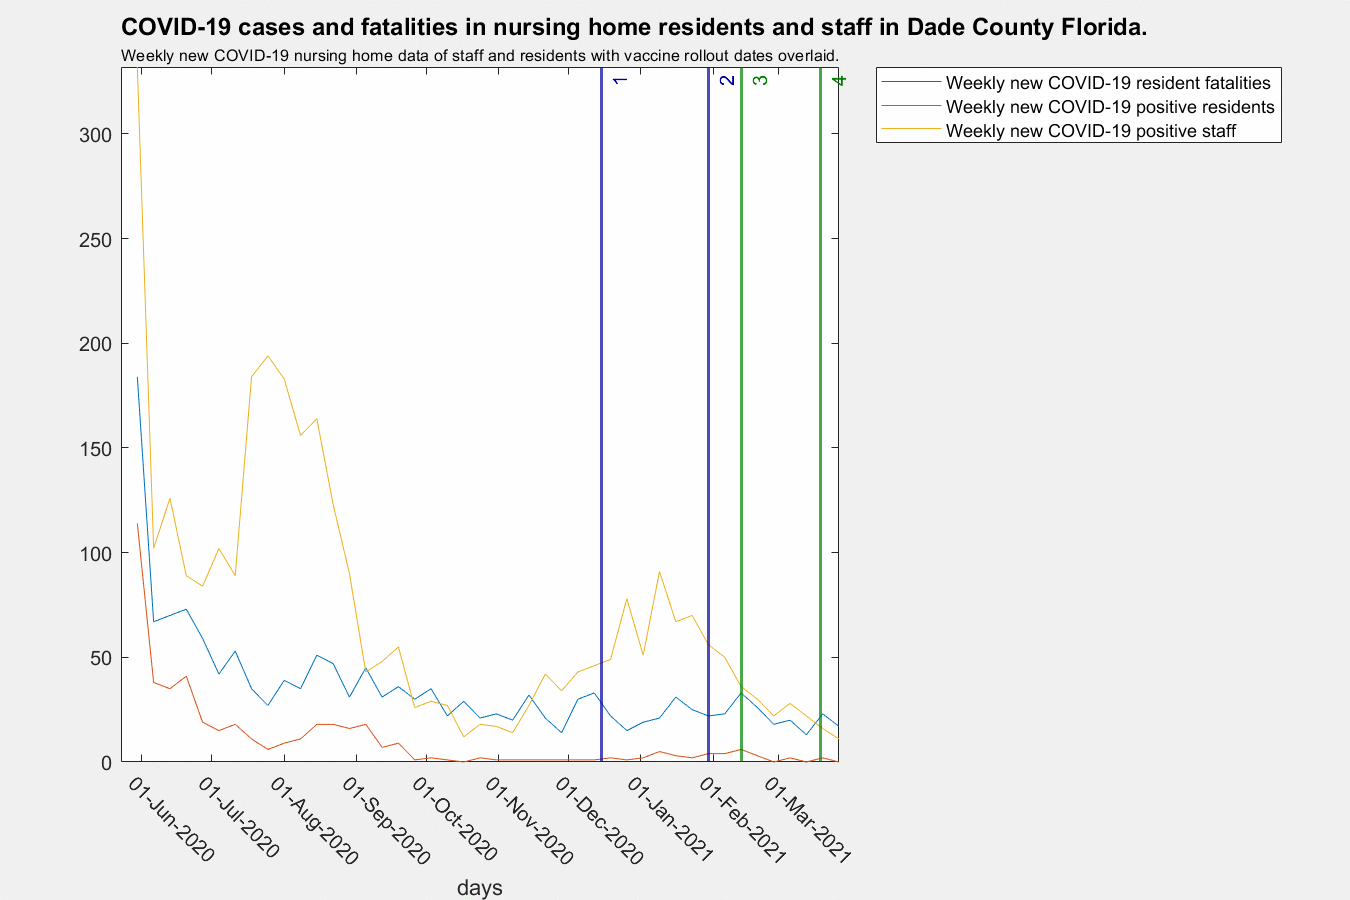
\includegraphics[width=\linewidth]{images/dade_nursing_home_with_vaccine.png}
	\caption{Nearly 4 weeks after COVID-19 vaccine distribution begins, new COVID-19 cases in nursing home staff begin to decline in Dade County Florida, while COVID-19 cases and fatalities in nursing home residents remain constant with a slight display in decline approximately 1 month after staff decline. }
	\label{fig:images/dade_nursing_home_with_vaccineLabel}
\end{figure}

\begin{figure}[H]
	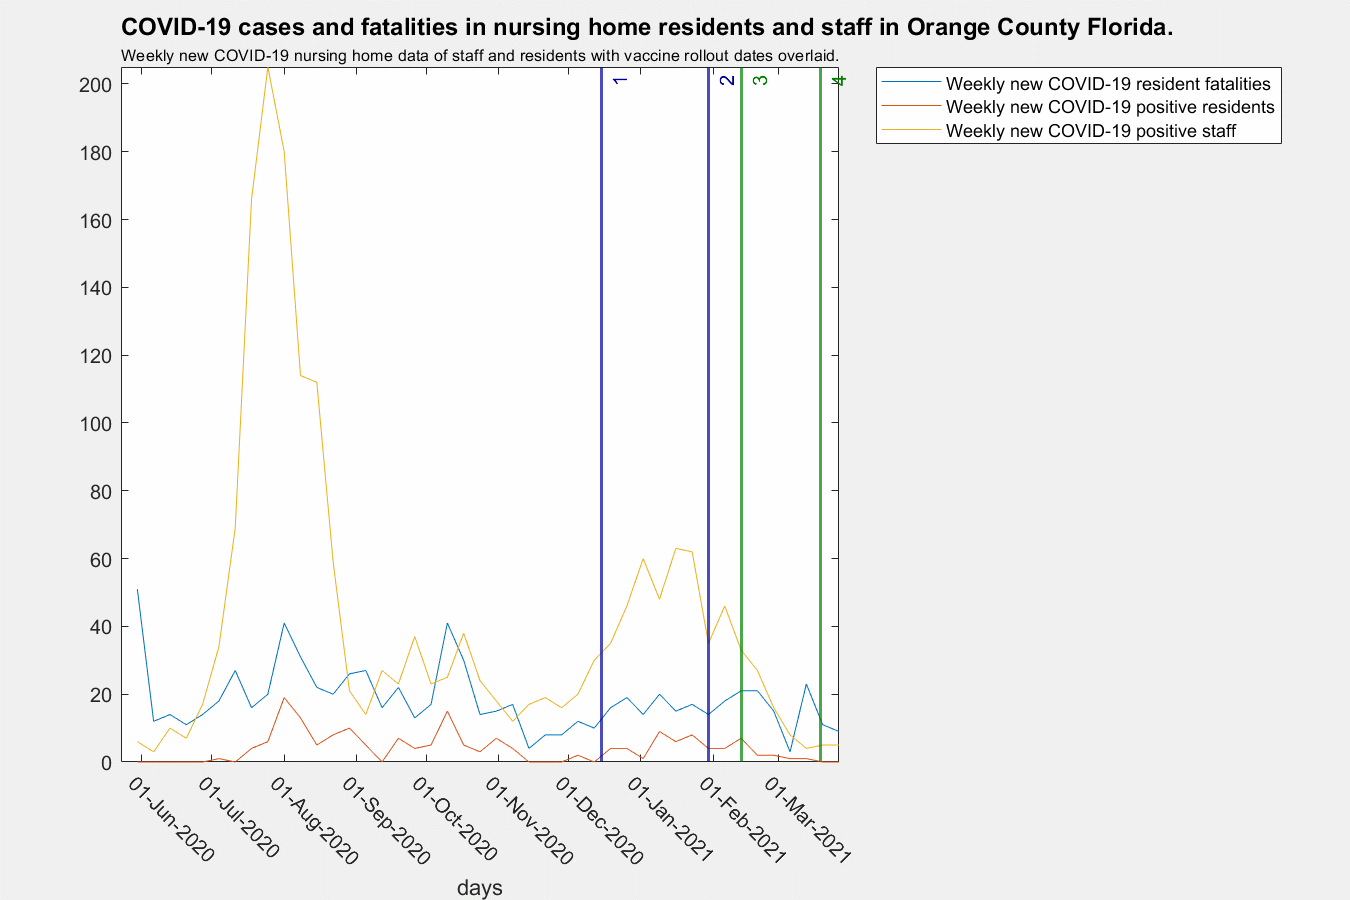
\includegraphics[width=\linewidth]{images/orange_nursing_home_with_vaccine.png}
	\caption{Approximately 5 weeks after the start of COVID-19 vaccine distribution, new COVID-19 cases in nursing home staff begin to decline in Orange County, Florida, while COVID-19 cases and fatalities in nursing home residents decline approximately 1 month after staff decline. }
	\label{fig:images/orange_nursing_home_with_vaccineLabel}
\end{figure}

\begin{figure}[H]
	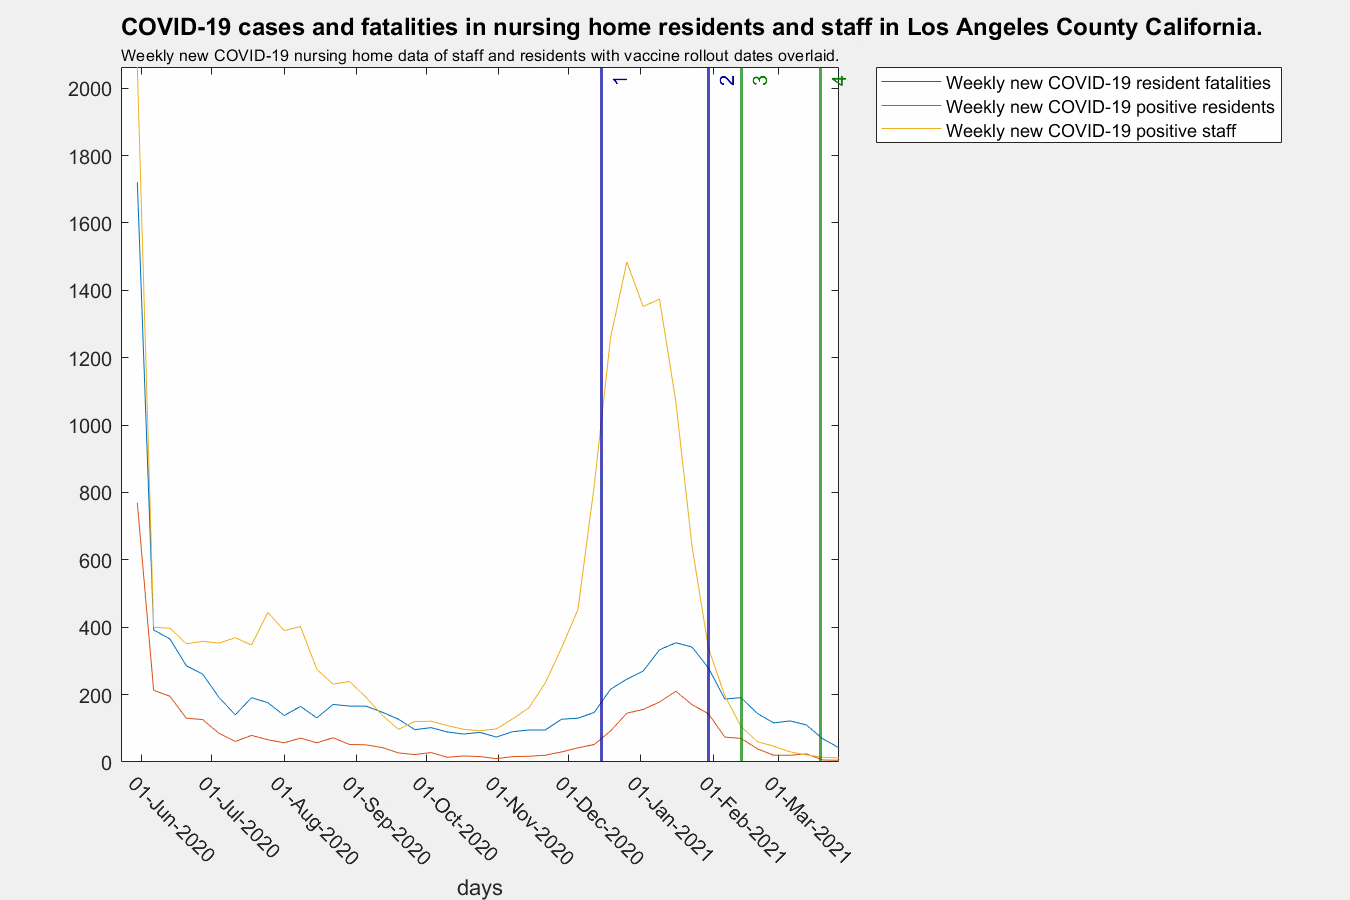
\includegraphics[width=\linewidth]{images/losangeles_nursing_home_with_vaccine.png}
	\caption{The release of the first COVID-19 vaccine is followed by a reduction in new COVID-19 cases in nursing home staff in Los Angeles County, California approximately 3 weeks after distribution; succeeded by a reduction in COVID-19 cases and fatalities in nursing home residents approximately 1 week later. }
	\label{fig:images/losangeles_nursing_home_with_vaccineLabel}
\end{figure}

\begin{figure}[H]
	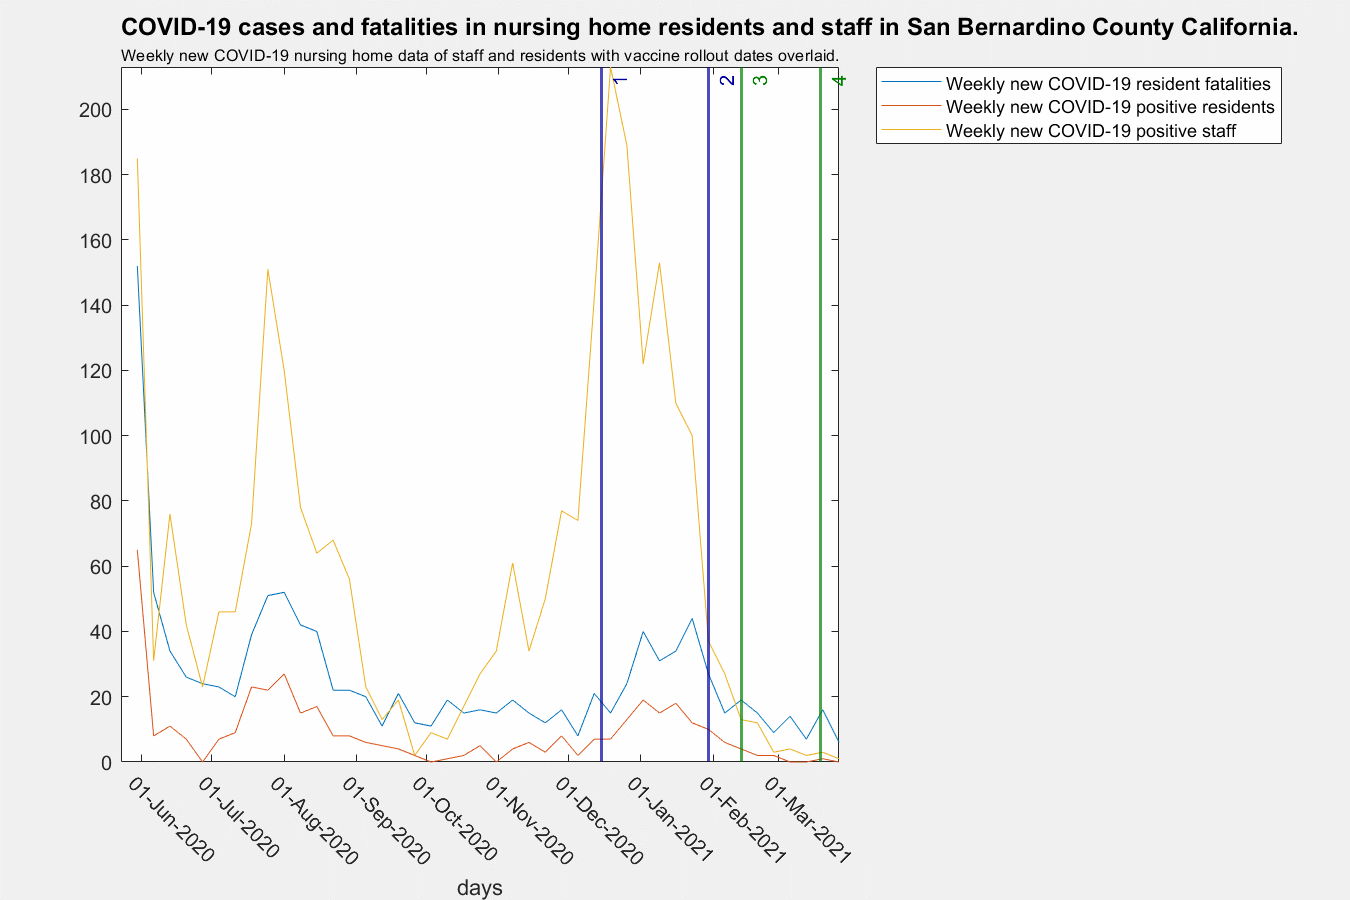
\includegraphics[width=\linewidth]{images/sanbernardino_nursing_home_with_vaccine.png}
	\caption{The release of the first COVID-19 vaccine is followed by a reduction in new COVID-19 cases in nursing home staff in San Bernardino County, California within 3 weeks, followed by a decline in COVID-19 cases and fataities in nursing home staff approximately 1 week later. }
	\label{fig:images/sanbernardino_nursing_home_with_vaccineLabel}
\end{figure}

\begin{figure}[H]
	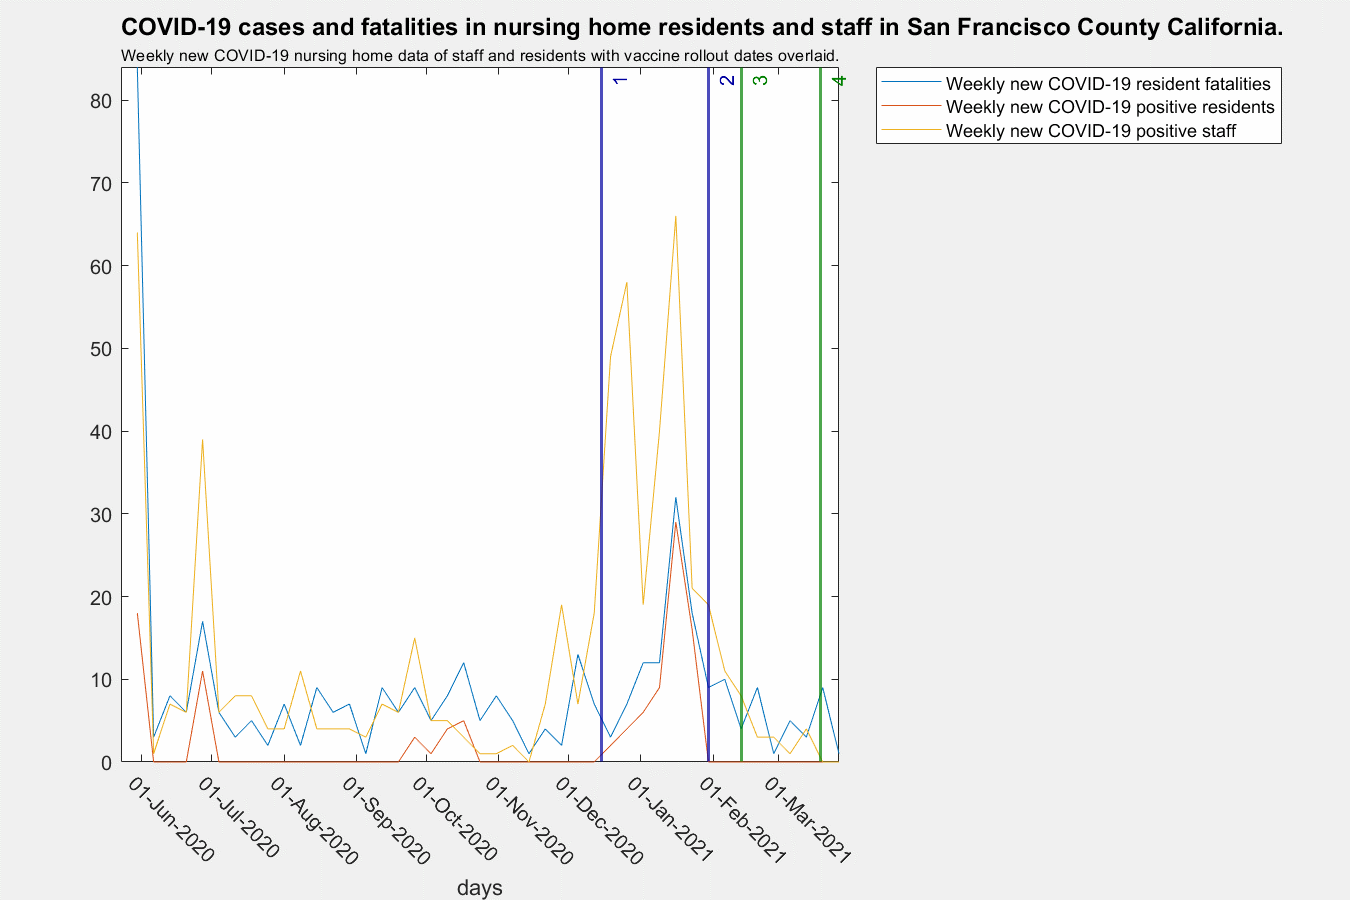
\includegraphics[width=\linewidth]{images/sanfrancisco_nursing_home_with_vaccine.png}
	\caption{Approximately 4 weeks after the distribution of the first COVID-19 vaccine, new COVID-19 cases in nursing home staff in San Francisco County, California begin to decline, followed by a decline in COVID-19 cases and fatalities in nursing home residents less than one week later.  }
	\label{fig:images/sanfrancisco_nursing_home_with_vaccineLabel}
\end{figure}

\begin{figure}[H]
	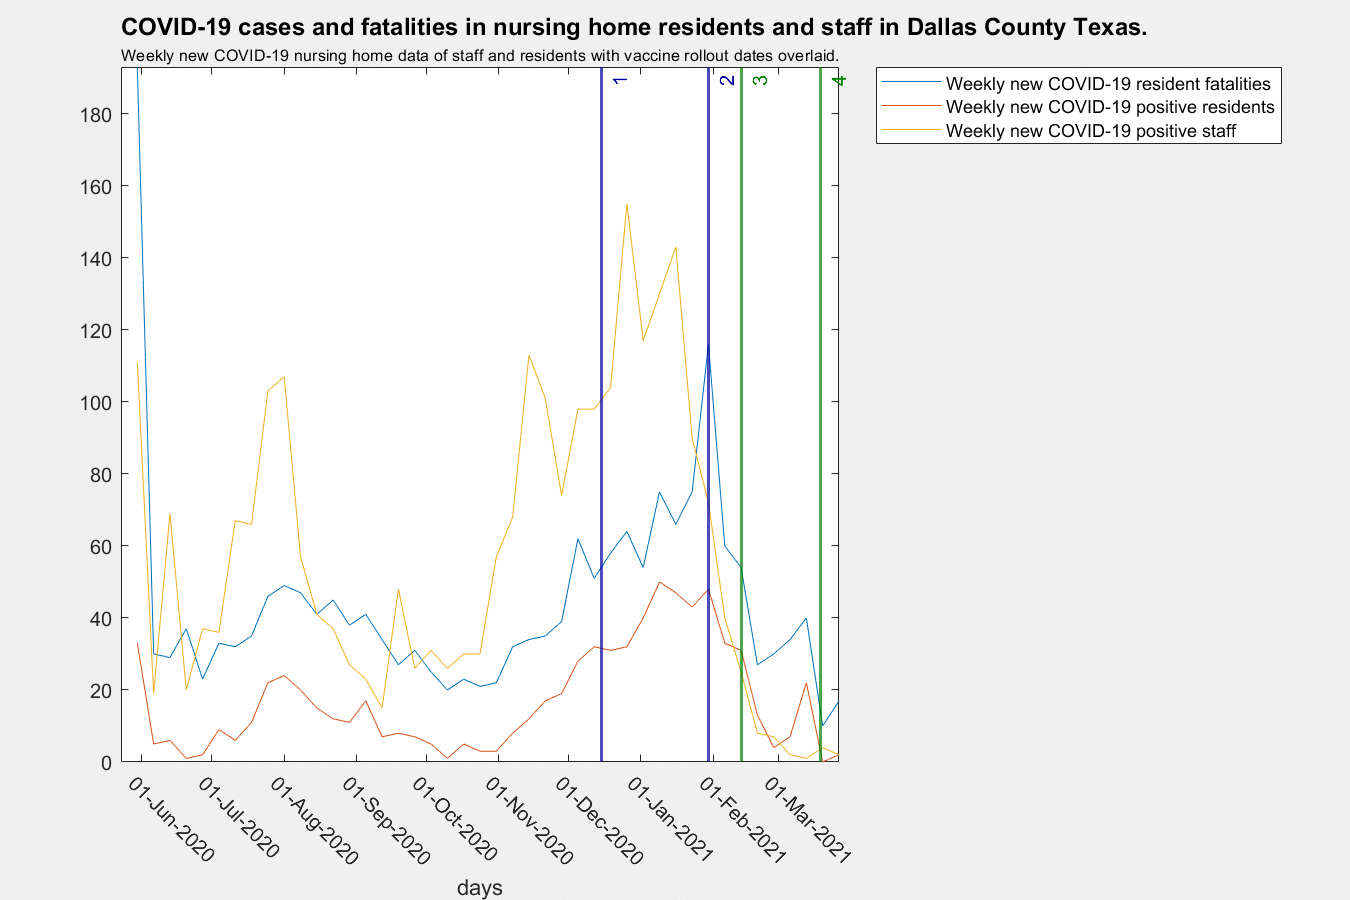
\includegraphics[width=\linewidth]{images/dallas_nursing_home_with_vaccine.png}
	\caption{New COVID-19 cases in nursing home staff in Dallas County, Texas begin to decline approximately 4 weeks after the distribution of the first COVID-19 vaccine, followed by the decline in COVID-19 cases and fatalities in nursing home residents approximately 2 weeks later.  }
	\label{fig:images/dallas_nursing_home_with_vaccineLabel}
\end{figure}

\begin{figure}[H]
	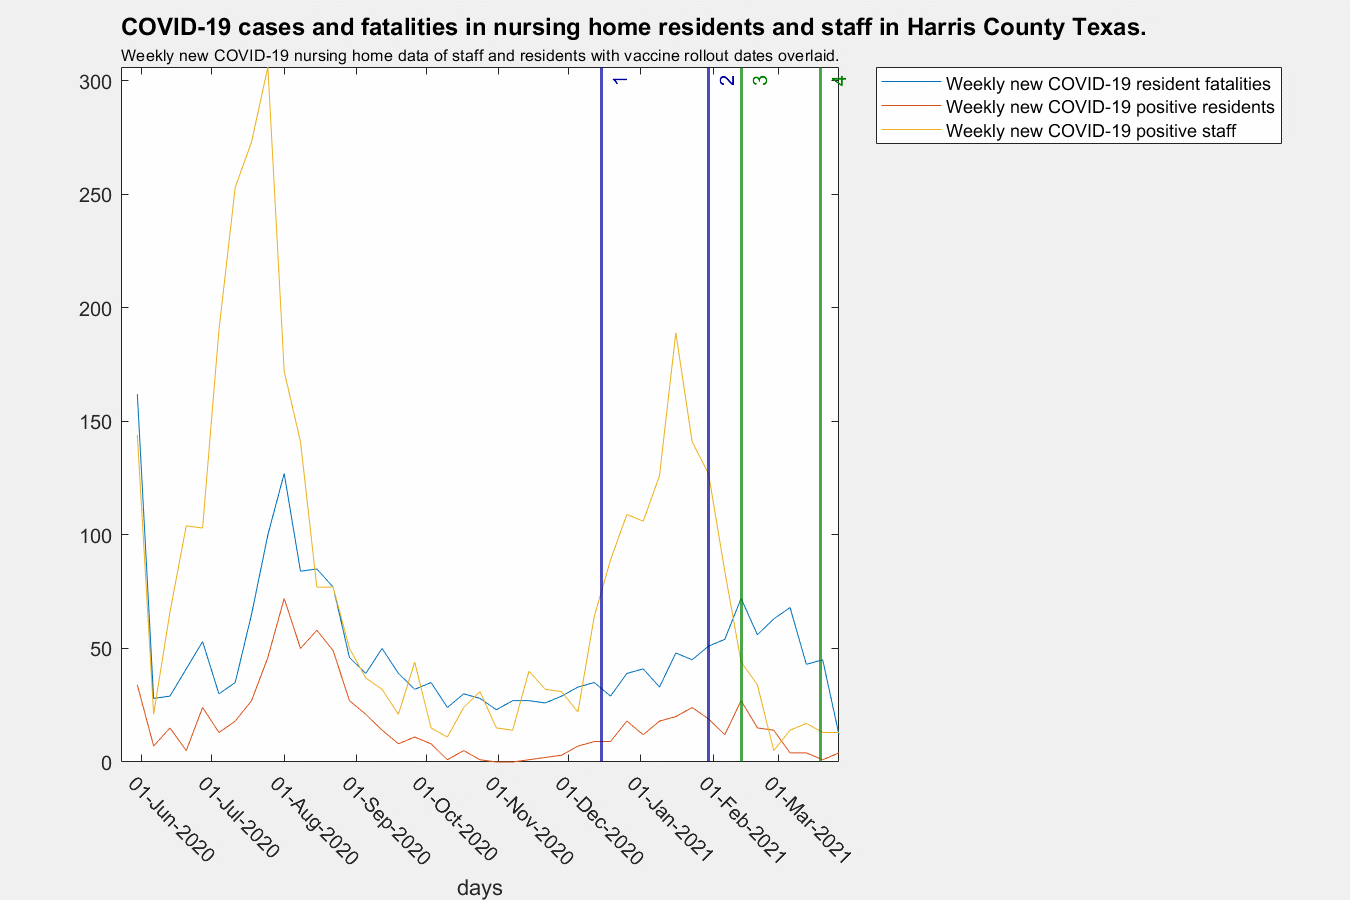
\includegraphics[width=\linewidth]{images/harris_nursing_home_with_vaccine.png}
	\caption{New COVID-19 cases in nursing home staff in Harris County, Texas begin to decline approximately 5 weeks after the distribution of the first COVID-19 vaccine, followed by the decline in COVID-19 cases and fatalities in nursing home residents approximately 2 weeks later. }
	\label{fig:images/harris_nursing_home_with_vaccineLabel}
\end{figure}

\begin{figure}[H]
	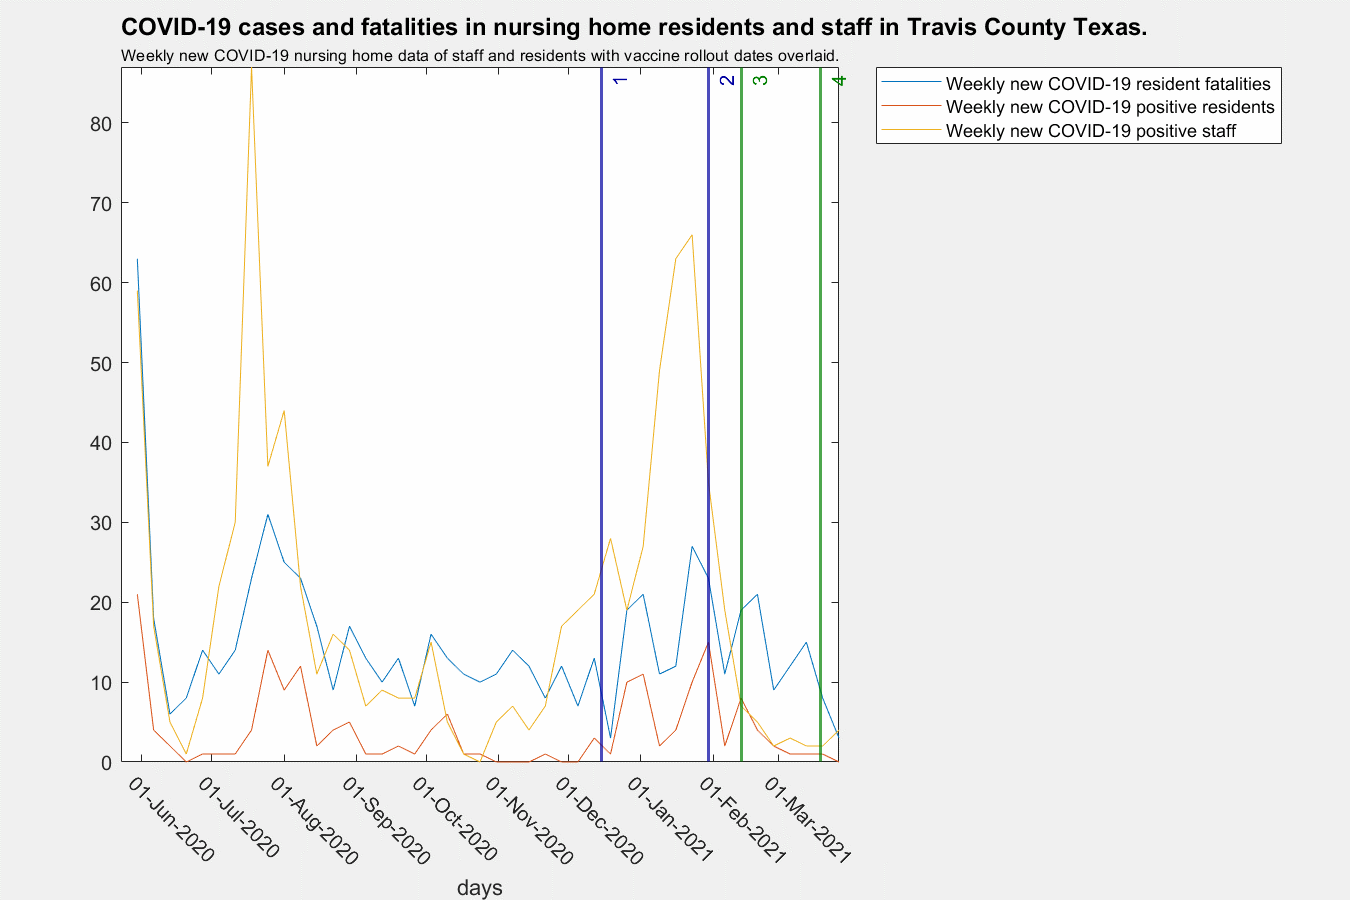
\includegraphics[width=\linewidth]{images/travis_nursing_home_with_vaccine.png}
	\caption{New COVID-19 cases in nursing home staff in Travis County, Texas begin to decline approximately 5 weeks after the distribution of the first COVID-19 vaccine, followed by the decline in COVID-19 cases and fatalities in nursing home residents approximately 2 weeks later. }
	\label{fig:images/travis_nursing_home_with_vaccineLabel}
\end{figure}

\subsection{Vaccinations in general public 65+ and in assisted living facility residents}

\begin{figure}[H]
	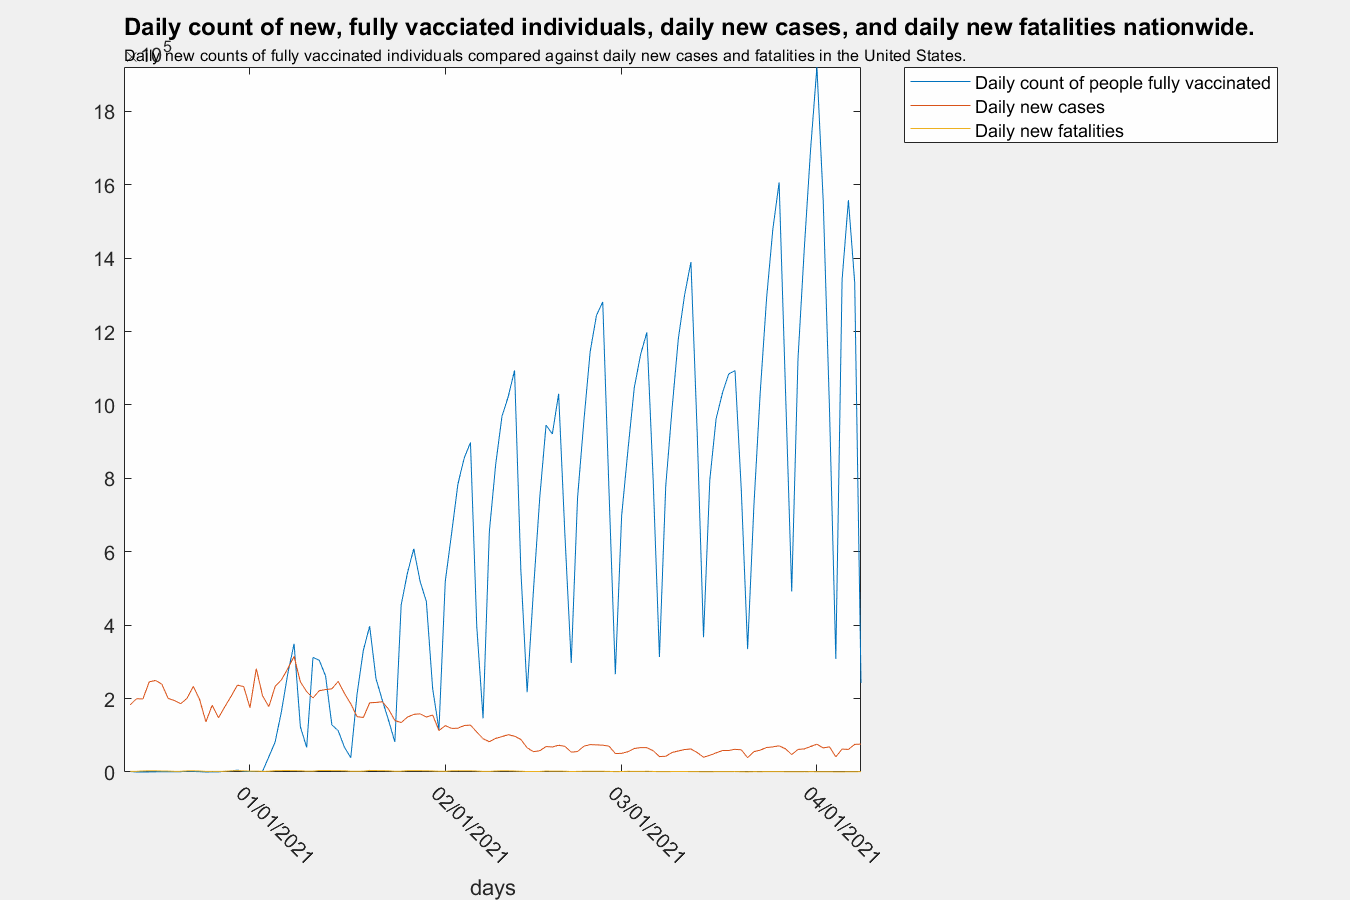
\includegraphics[width=\linewidth]{images/nationwide_fully_vaccinated.png}
	\caption{A national timeline of daily new cases and fatalities due to COVID-19, plotted with daily new vaccines. According to the figure, as the rate of daily, new vaccinated individuals increases, daily new COVID-19 cases and fatalities decreases.}
	\label{fig:images/nationwide_fully_vaccinatedLabel}
\end{figure}

\begin{figure}[H]
	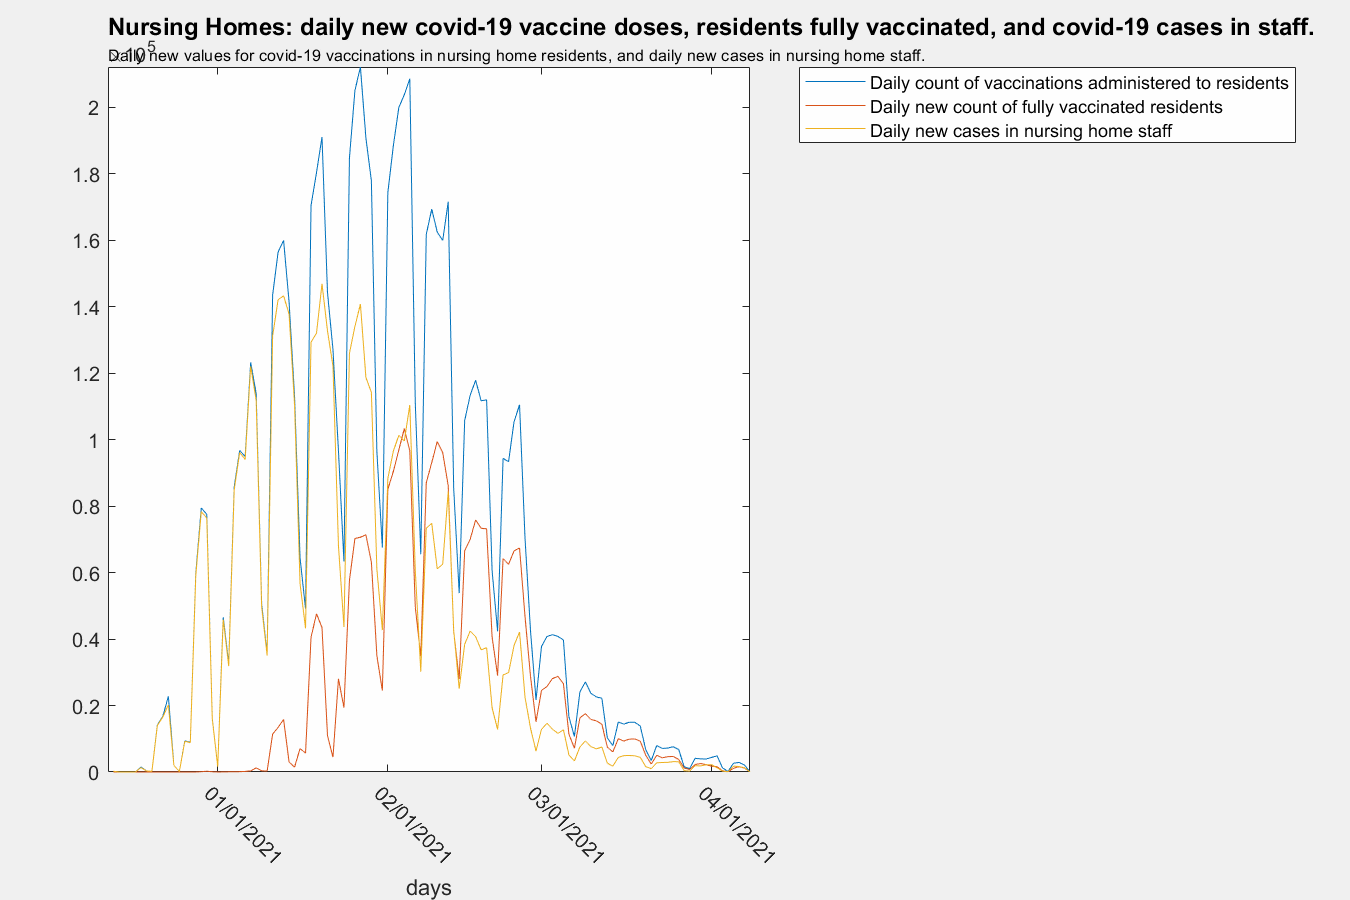
\includegraphics[width=\linewidth]{images/ltc_fully_vaccinated.png}
	\caption{A timeline of daily new COVID-19 vaccinations in long term care residents, daily count of new, fully vaccinated residents, and new COVID-19 cases in long term care staff.  }
	\label{fig:images/ltc_fully_vaccinatedLabel}
\end{figure}

\begin{figure}[H]
	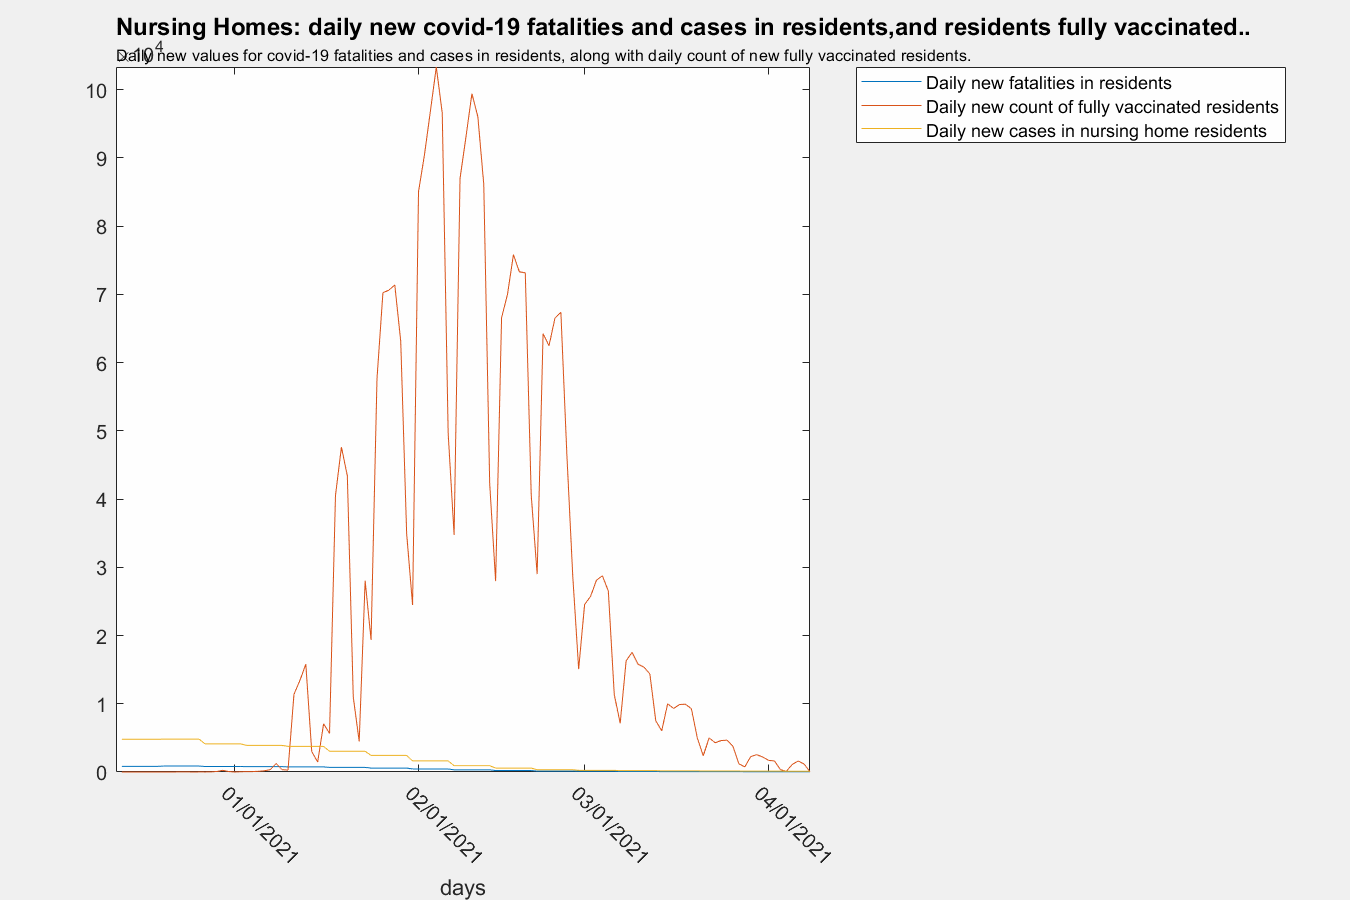
\includegraphics[width=\linewidth]{images/ltc_daily_cases.png}
	\caption{A timeline of daily new COVID-19 cases and fatalities in long term care residents with daily new residents fully vaccinated.}
	\label{fig:images/ltc_daily_casesLabel}
\end{figure}

\begin{figure}[H]
	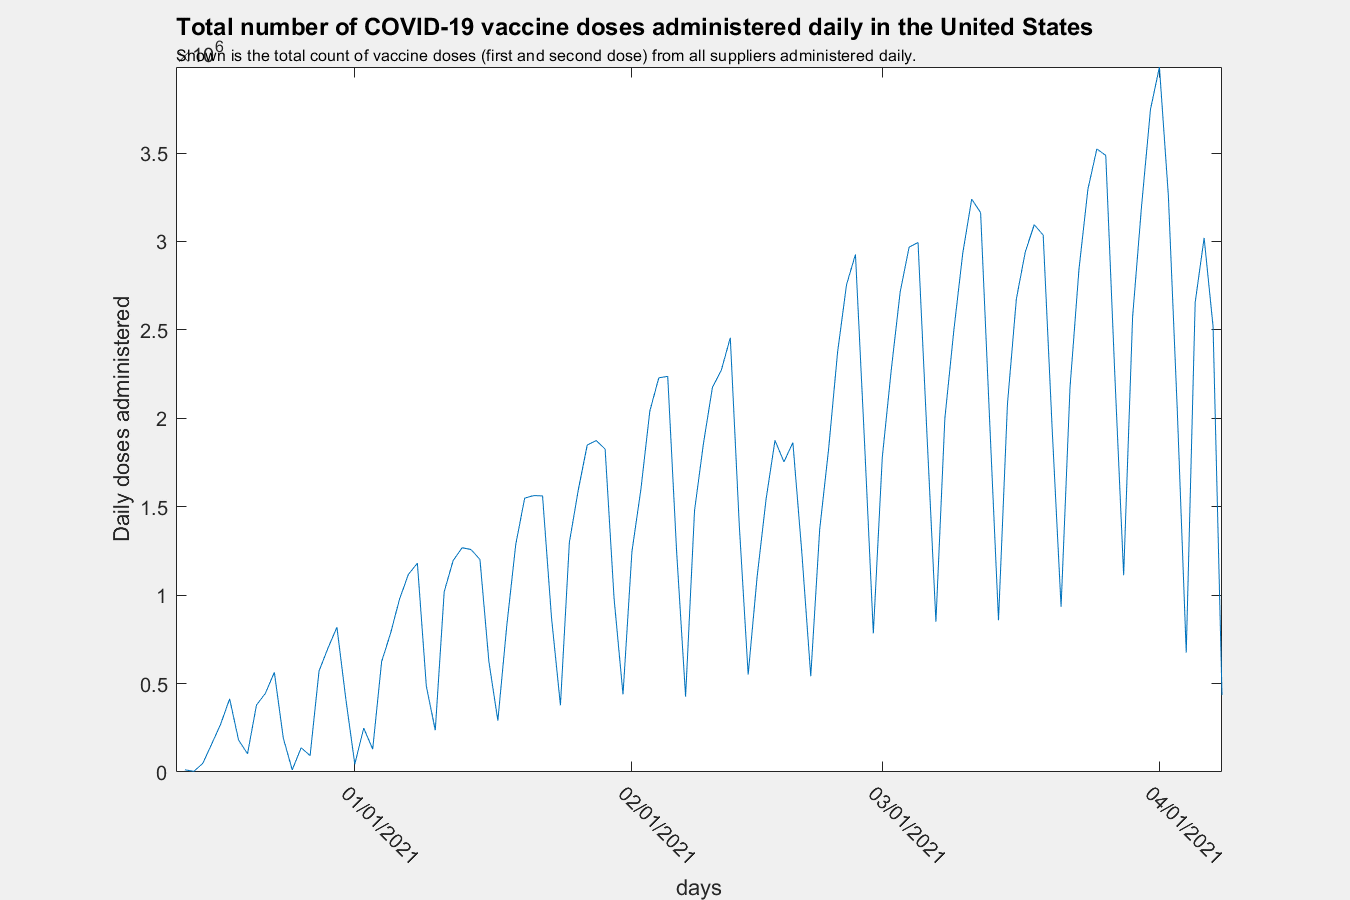
\includegraphics[width=\linewidth]{images/usa_daily_total_doses_unprocessed.png}
	\caption{Shown above is the daily count of COVID-19 vaccines administered daily in the United States. The count includes a first dose injection, a second dose injection, and a single-dose injection.}
	\label{fig:images/usa_daily_total_doses_unprocessedLabel}
\end{figure}

\begin{figure}[H]
	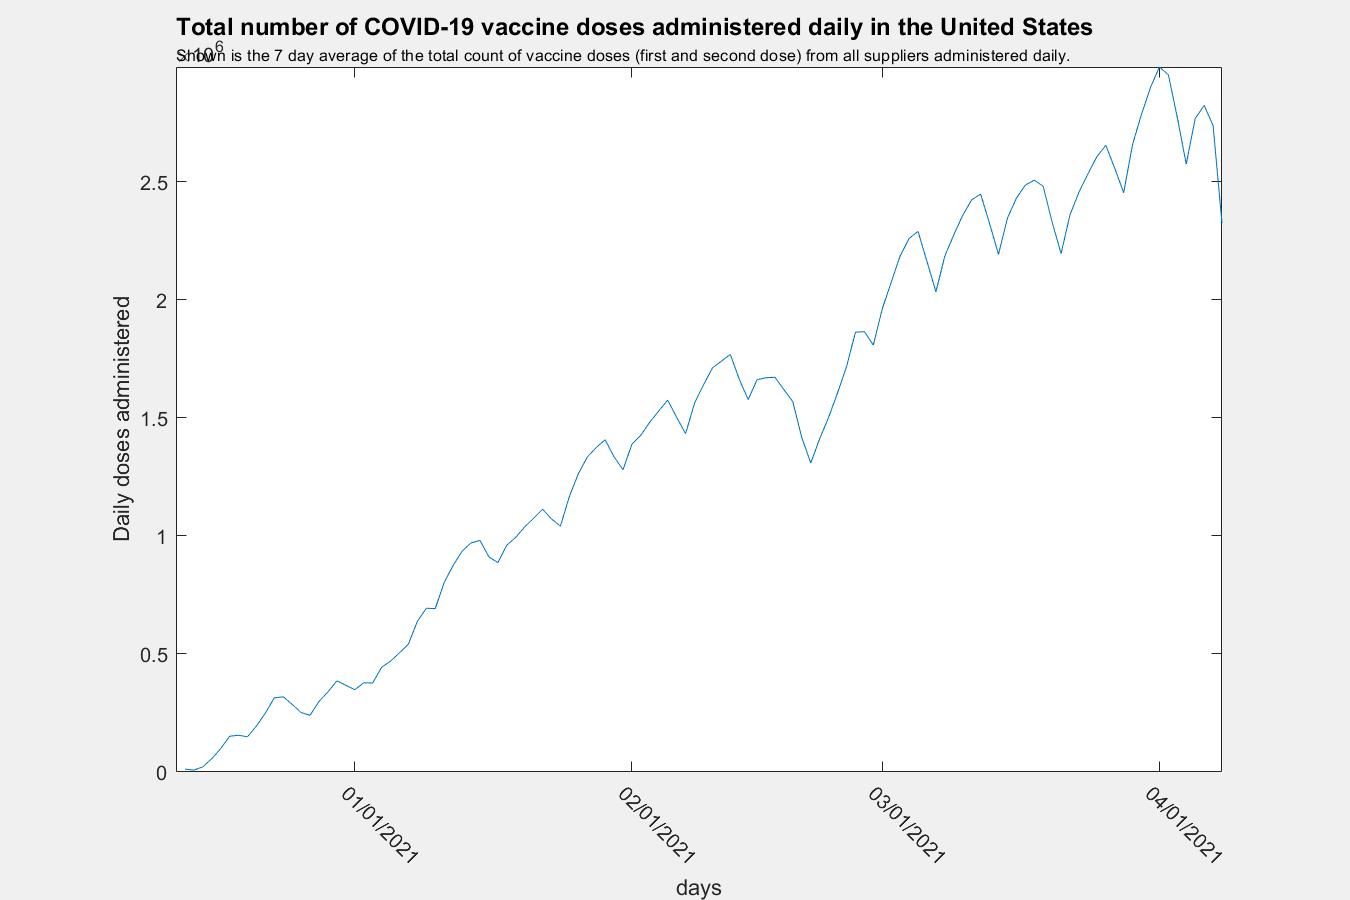
\includegraphics[width=\linewidth]{images/usa_daily_total_doses_processed.png}
	\caption{Shown above is the rolling 7 day average of the count of COVID-19 vaccines administered daily in the United States. The count includes a first dose injection, a second dose injection, and a single-dose injection.}
	\label{fig:images/usa_daily_total_doses_processedLabel}
\end{figure}

\begin{figure}[H]
	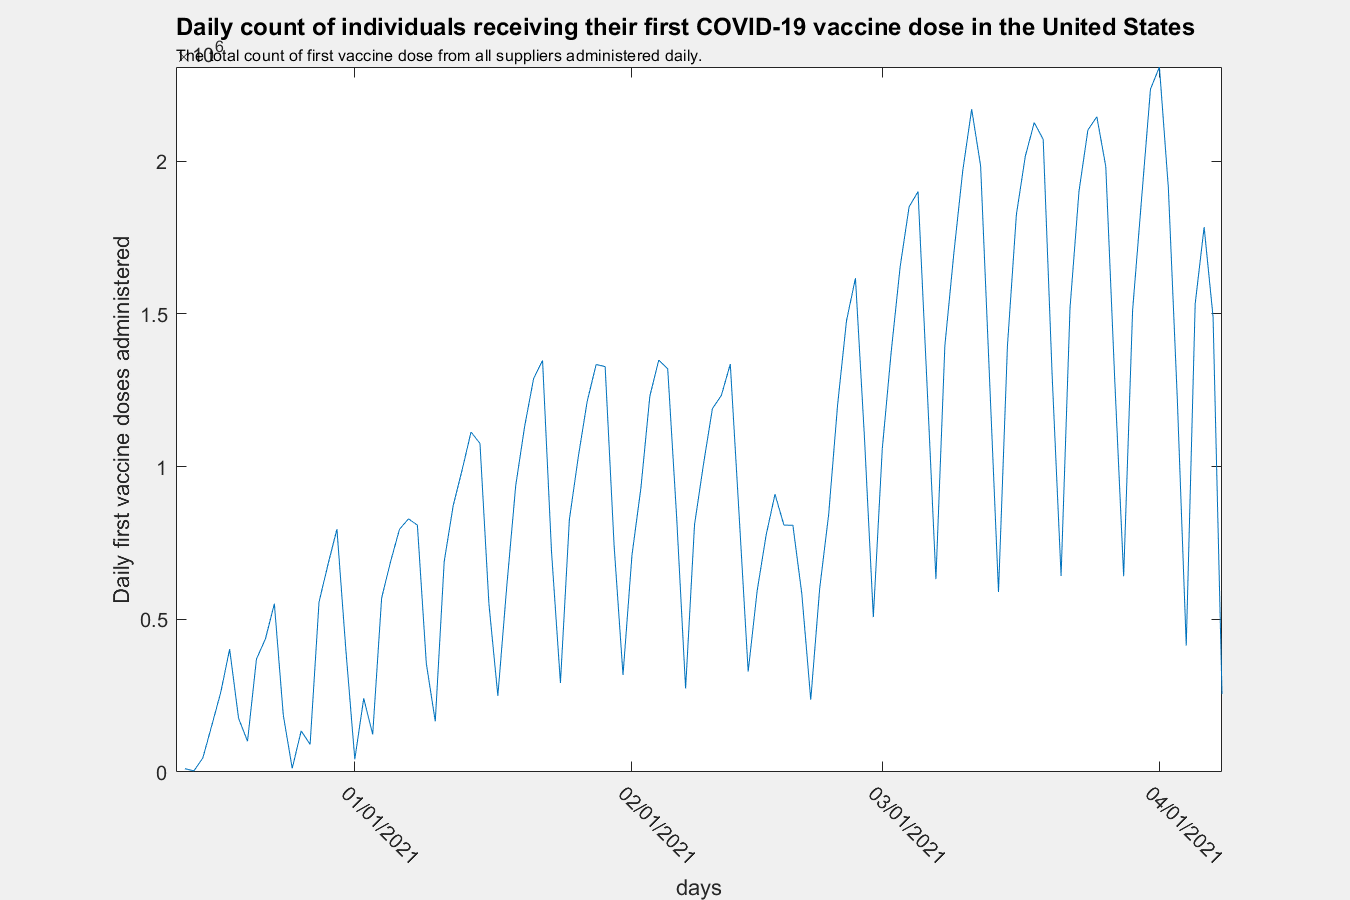
\includegraphics[width=\linewidth]{images/usa_daily_first_doses_unprocessed.png}
	\caption{Shown is the daily count of individuals receiving their first COVID-19 vaccine dose in the United States. }
	\label{fig:images/usa_daily_first_doses_unprocessedLabel}
\end{figure}

\begin{figure}[H]
	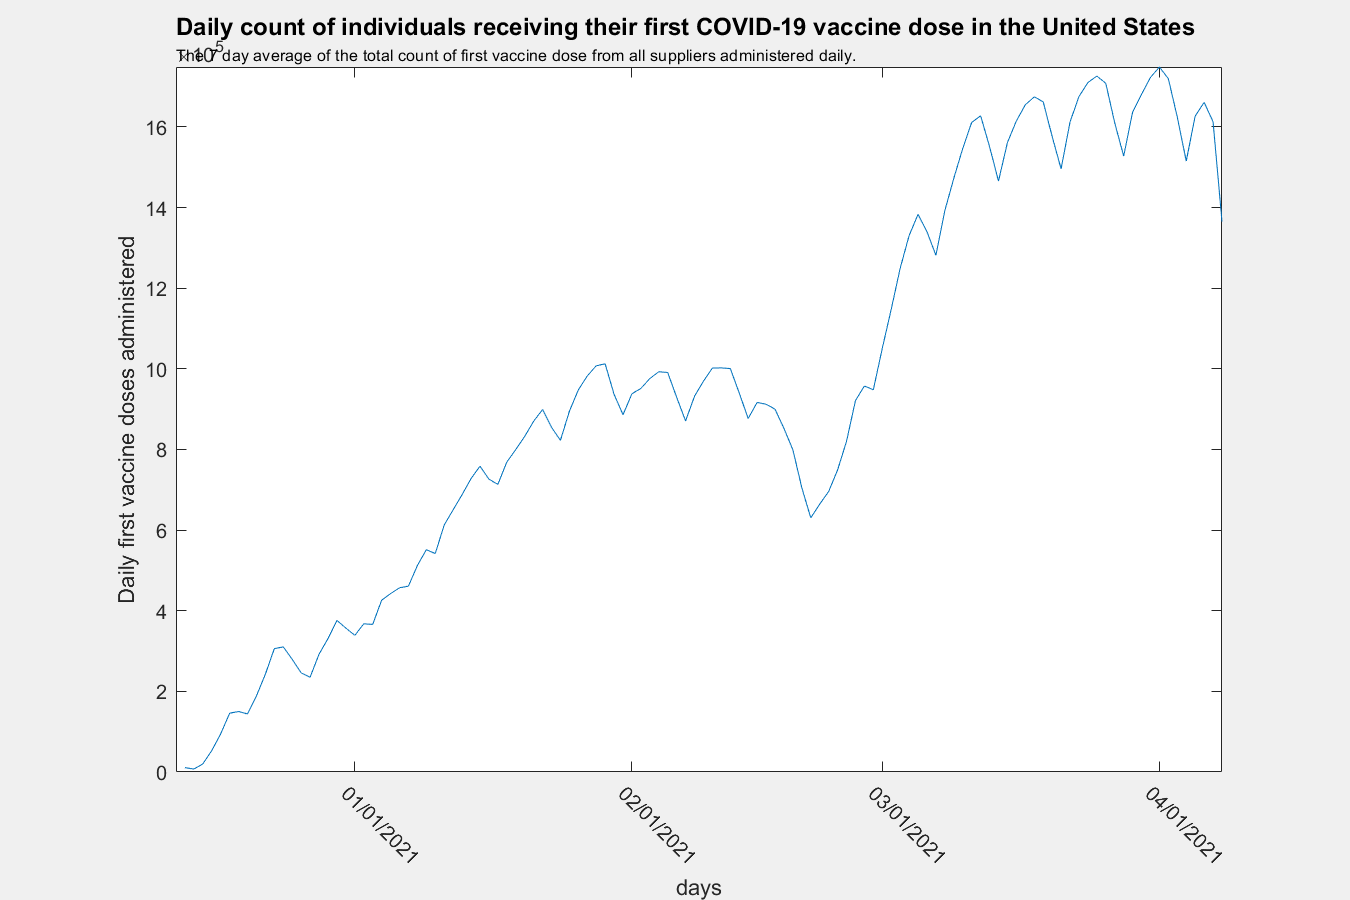
\includegraphics[width=\linewidth]{images/usa_daily_first_doses_processed.png}
	\caption{Shown is the rolling 7 day average of individuals receiving their first COVID-19 vaccine dose in the United States.}
	\label{fig:images/usa_daily_first_doses_processedLabel}
\end{figure}

\begin{figure}[H]
	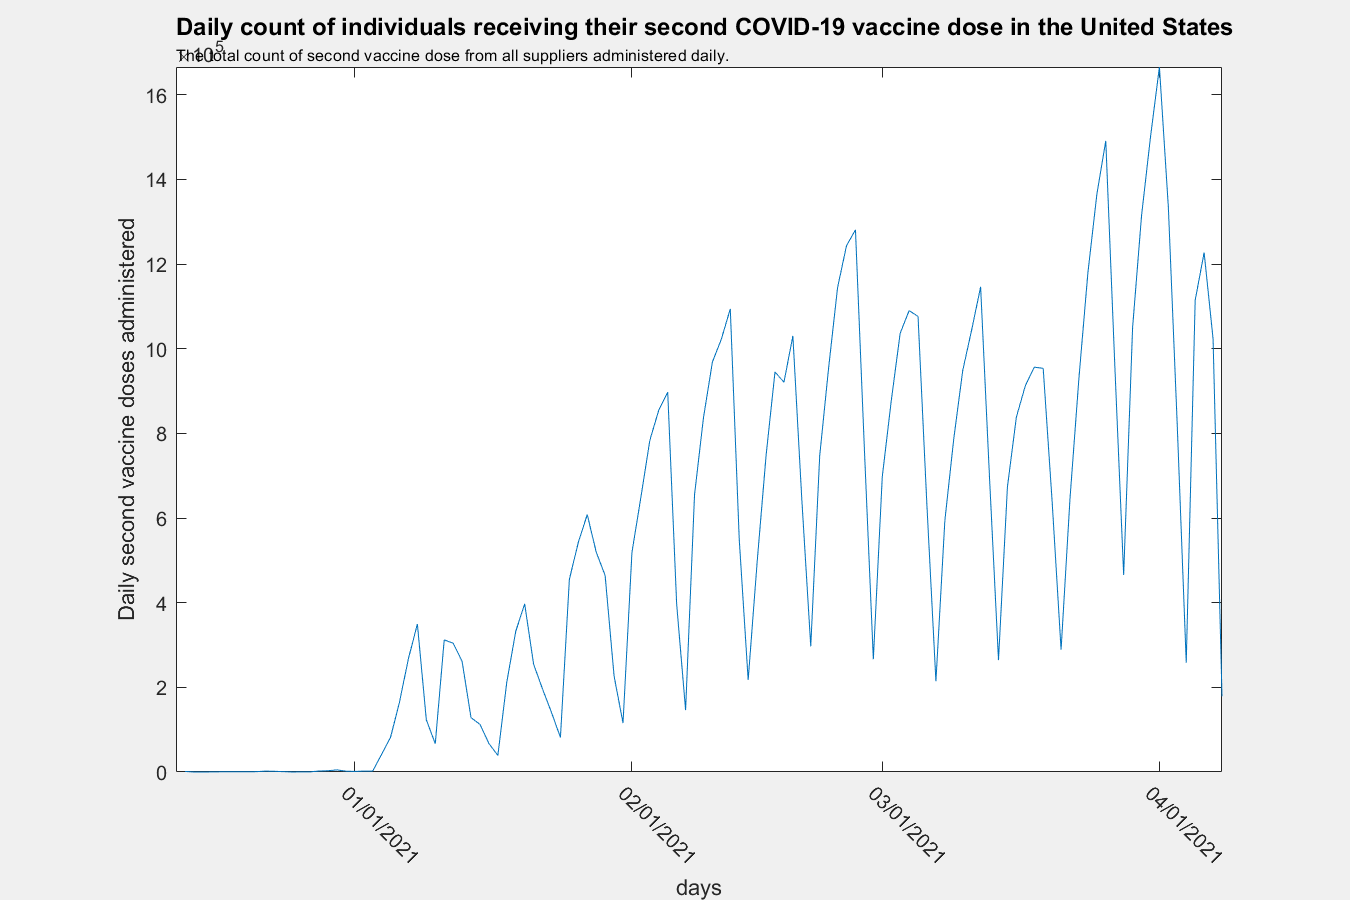
\includegraphics[width=\linewidth]{images/usa_daily_second_doses_unprocessed.png}
	\caption{Shown is the daily count of individuals receiving their second COVID-19 vaccine dose in the United States.}
	\label{fig:images/usa_daily_second_doses_unprocessedLabel}
\end{figure}

\begin{figure}[H]
	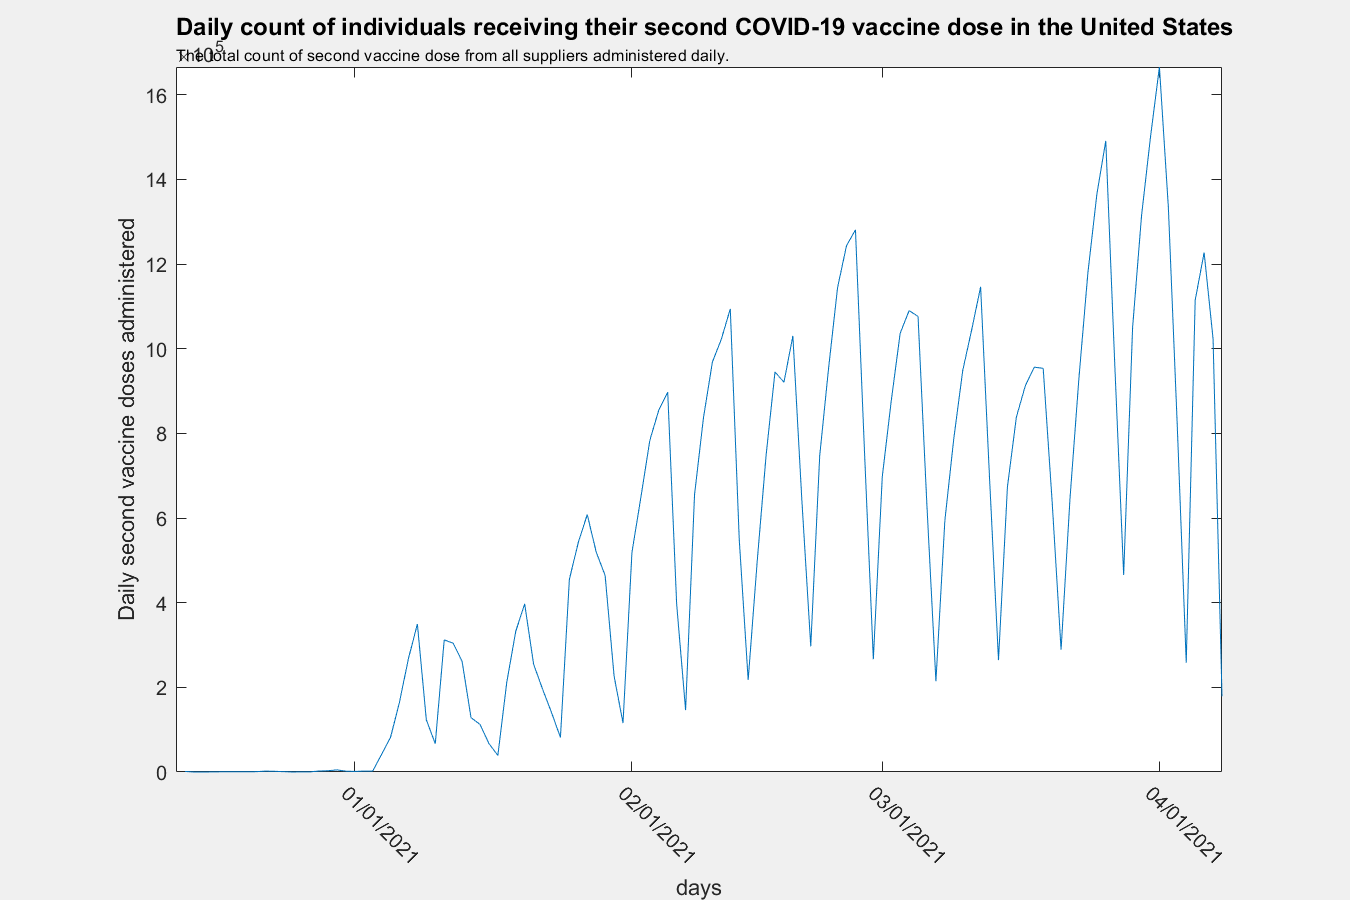
\includegraphics[width=\linewidth]{images/usa_daily_second_doses_unprocessed.png}
	\caption{Shown is the rolling 7 day average of individuals receiving their second COVID-19 vaccine dose in the United States.}
	\label{fig:images/usa_daily_second_doses_unprocessedLabel}
\end{figure}

\begin{figure}[H]
	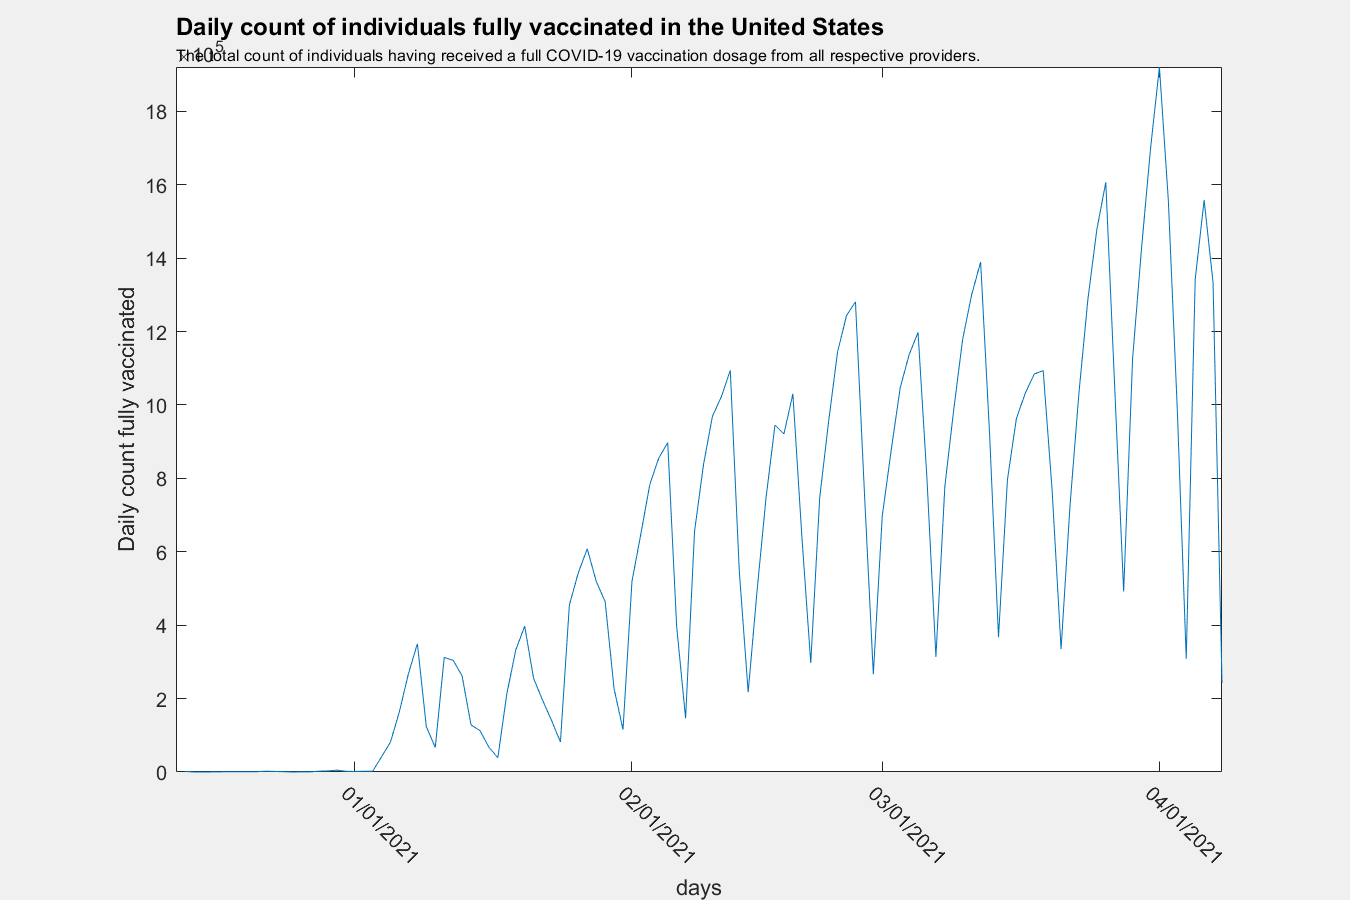
\includegraphics[width=\linewidth]{images/usa_daily_fully_vaccinated_unprocessed.png}
	\caption{Shown is the daily count of new individuas fully vaccinated in the United States. }
	\label{fig:images/usa_daily_fully_vaccinated_unprocessedLabel}
\end{figure}

\begin{figure}[H]
	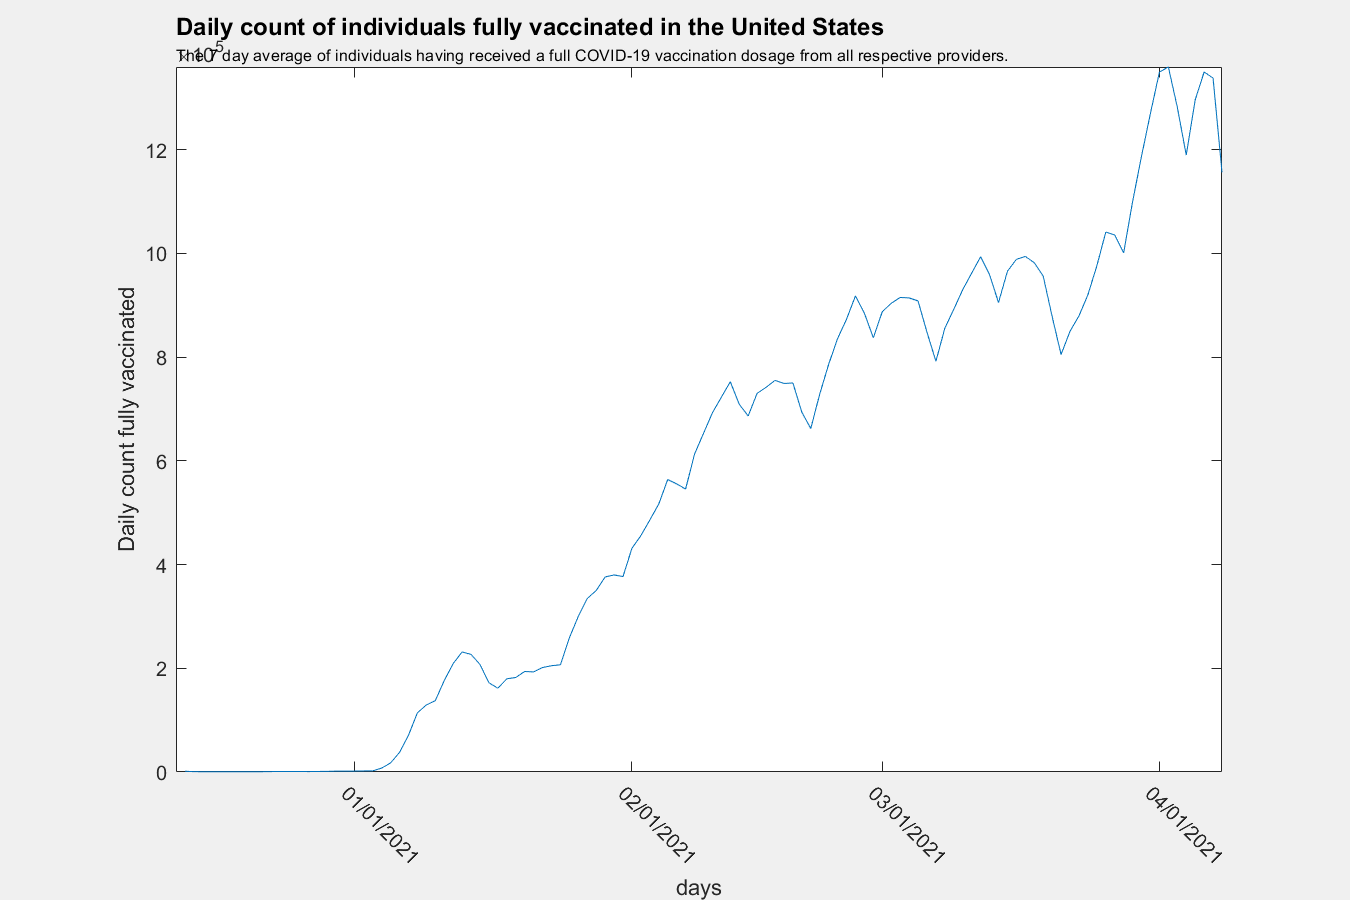
\includegraphics[width=\linewidth]{images/usa_daily_fully_vaccinated_processed.png}
	\caption{Shown is the rolling 7 day average of new individuas fully vaccinated in the United States.}
	\label{fig:images/usa_daily_fully_vaccinated_processedLabel}
\end{figure}

\begin{figure}[H]
	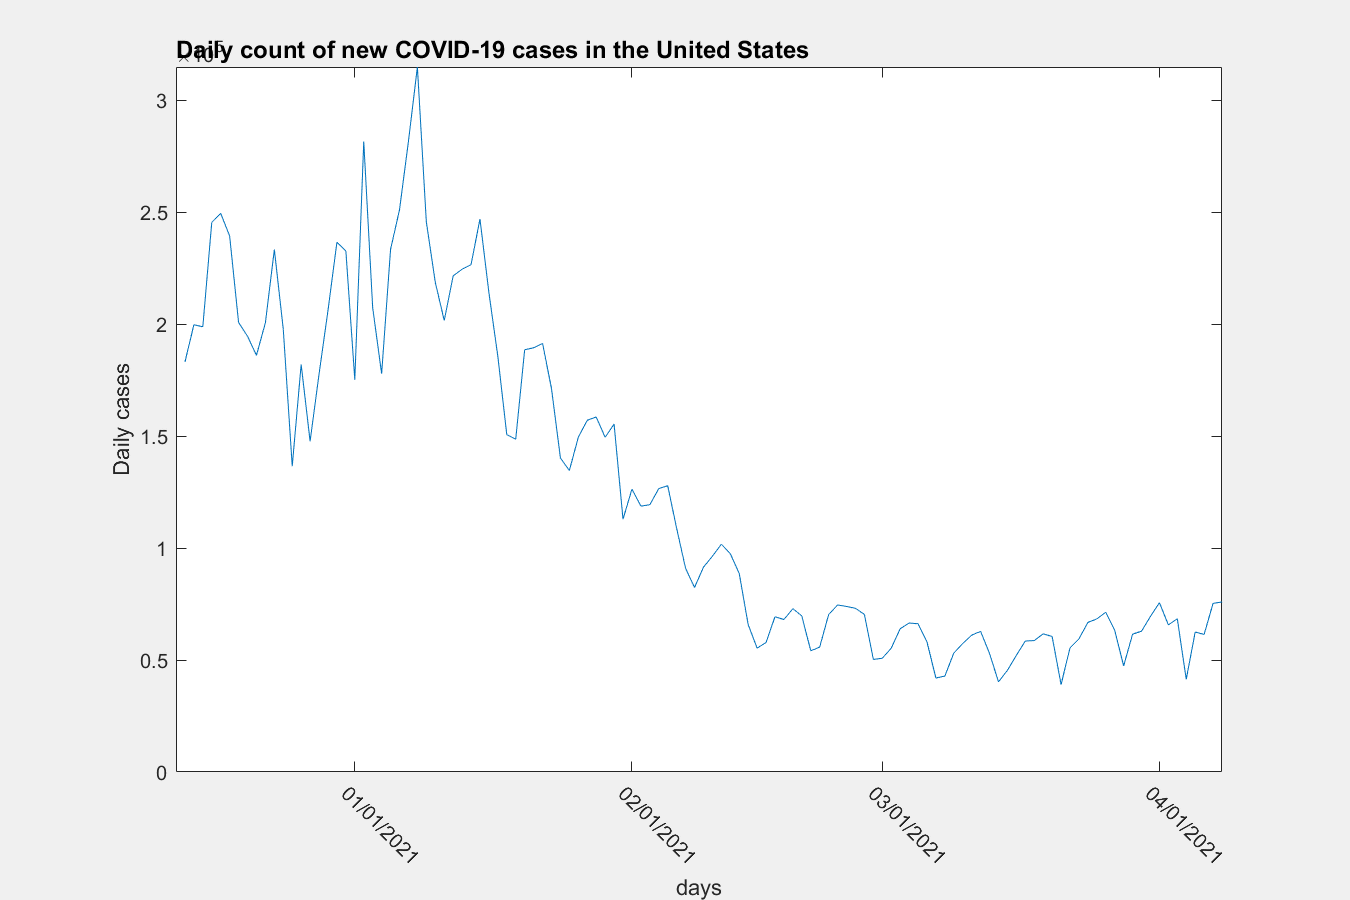
\includegraphics[width=\linewidth]{images/usa_daily_cases_unprocessed.png}
	\caption{Shown is the daily new count of individuals in the United States who have contracted COVID-19.}
	\label{fig:images/usa_daily_cases_unprocessedLabel}
\end{figure}

\begin{figure}[H]
	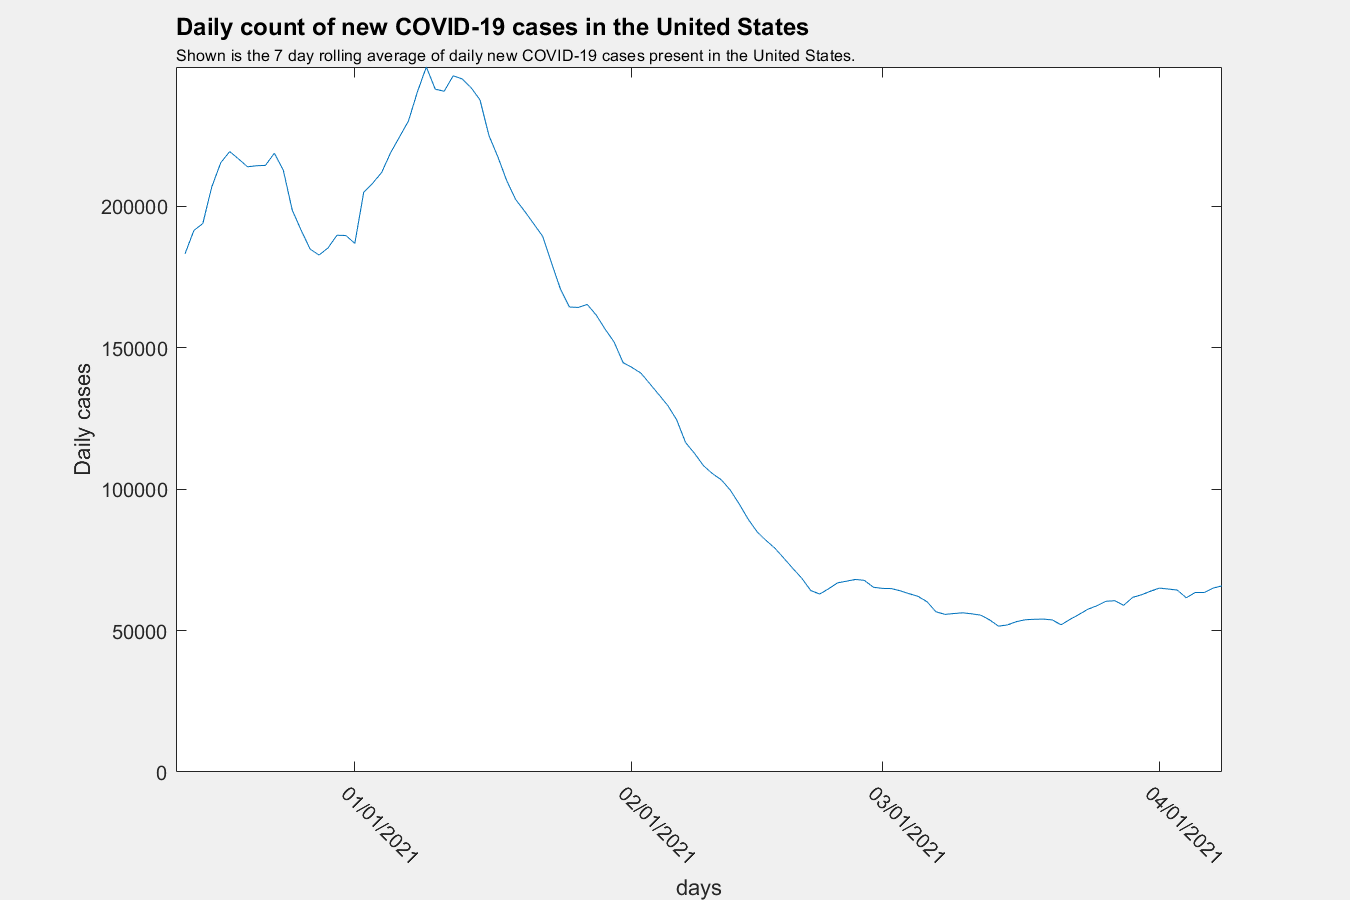
\includegraphics[width=\linewidth]{images/usa_daily_cases_processed.png}
	\caption{Shown is the rolling 7 day average of individuals in the United States who have contracted COVID-19.}
	\label{fig:images/usa_daily_cases_processedLabel}
\end{figure}

\begin{figure}[H]
	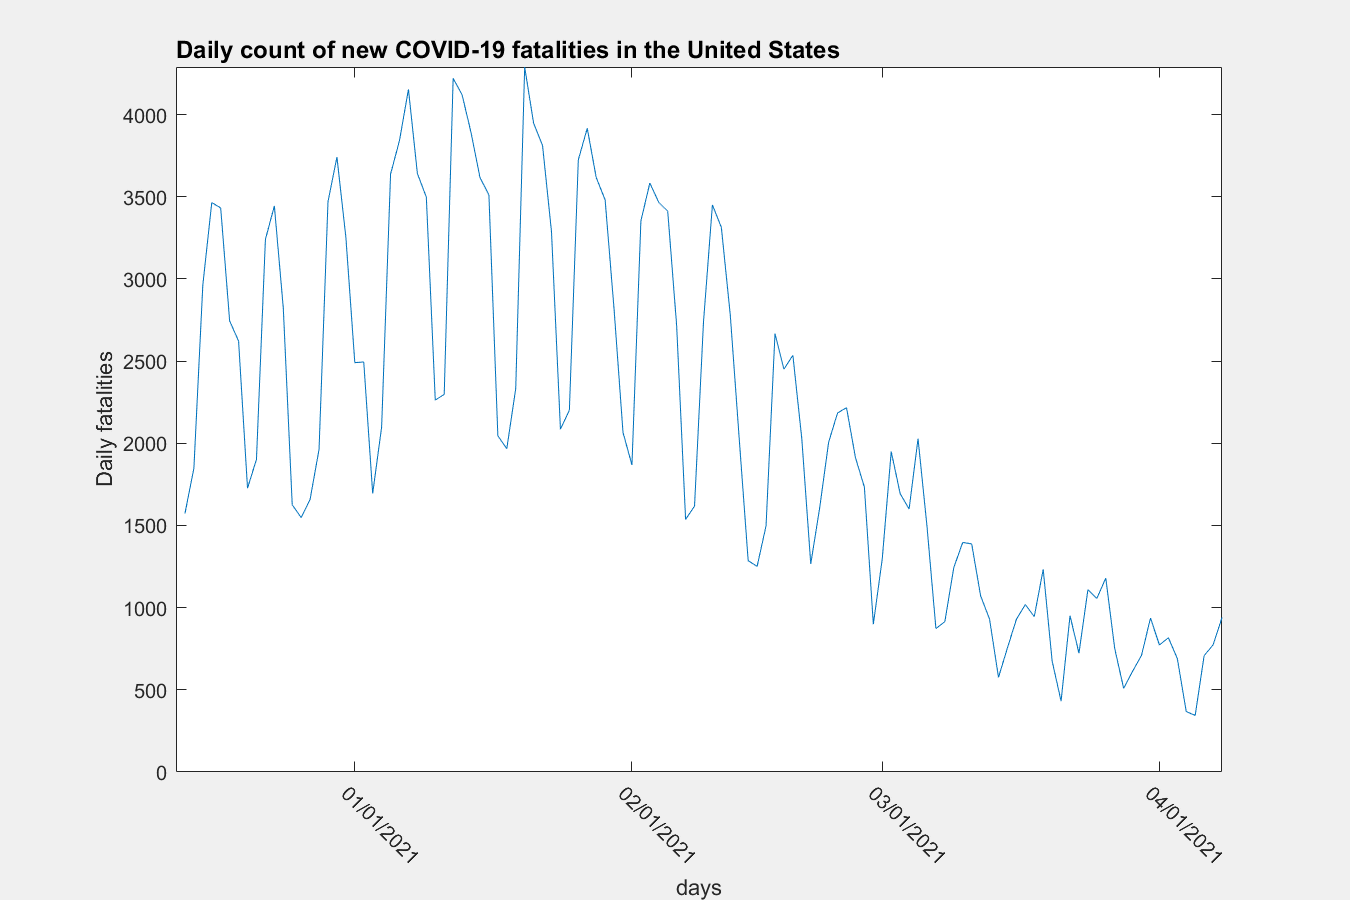
\includegraphics[width=\linewidth]{images/usa_daily_fatalities_unprocessed.png}
	\caption{Shown is the daily new count of deceased individuals in the United States who have died due to COVID-19.}
	\label{fig:images/usa_daily_fatalities_unprocessedLabel}
\end{figure}

\begin{figure}[H]
	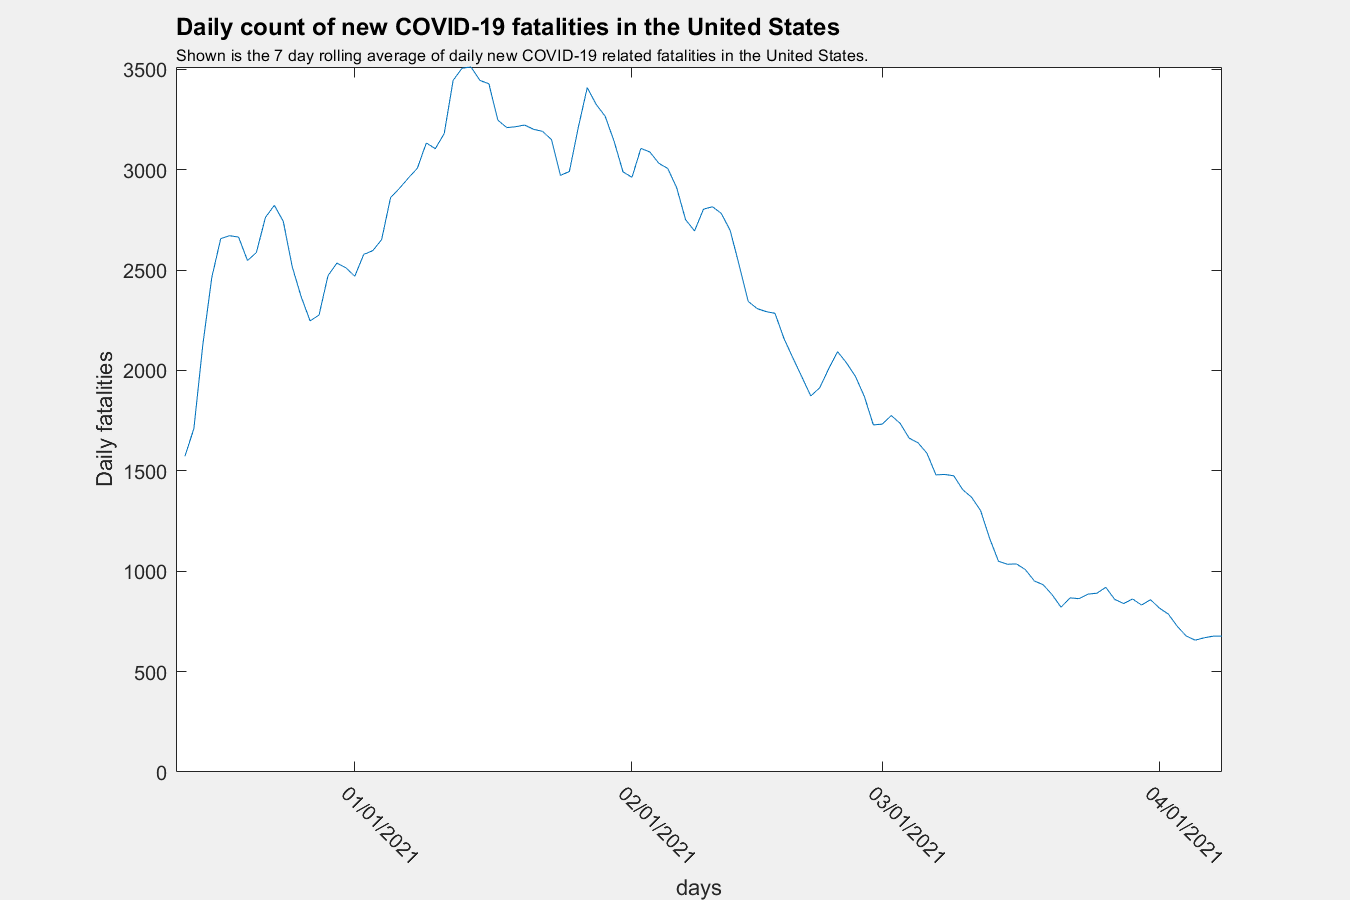
\includegraphics[width=\linewidth]{images/usa_daily_fatalities_processed.png}
	\caption{Shown is the daily new count of deceased individuals in the United States who have died due to COVID-19.}
	\label{fig:images/usa_daily_fatalities_processedLabel}
\end{figure}

\begin{figure}[H]
	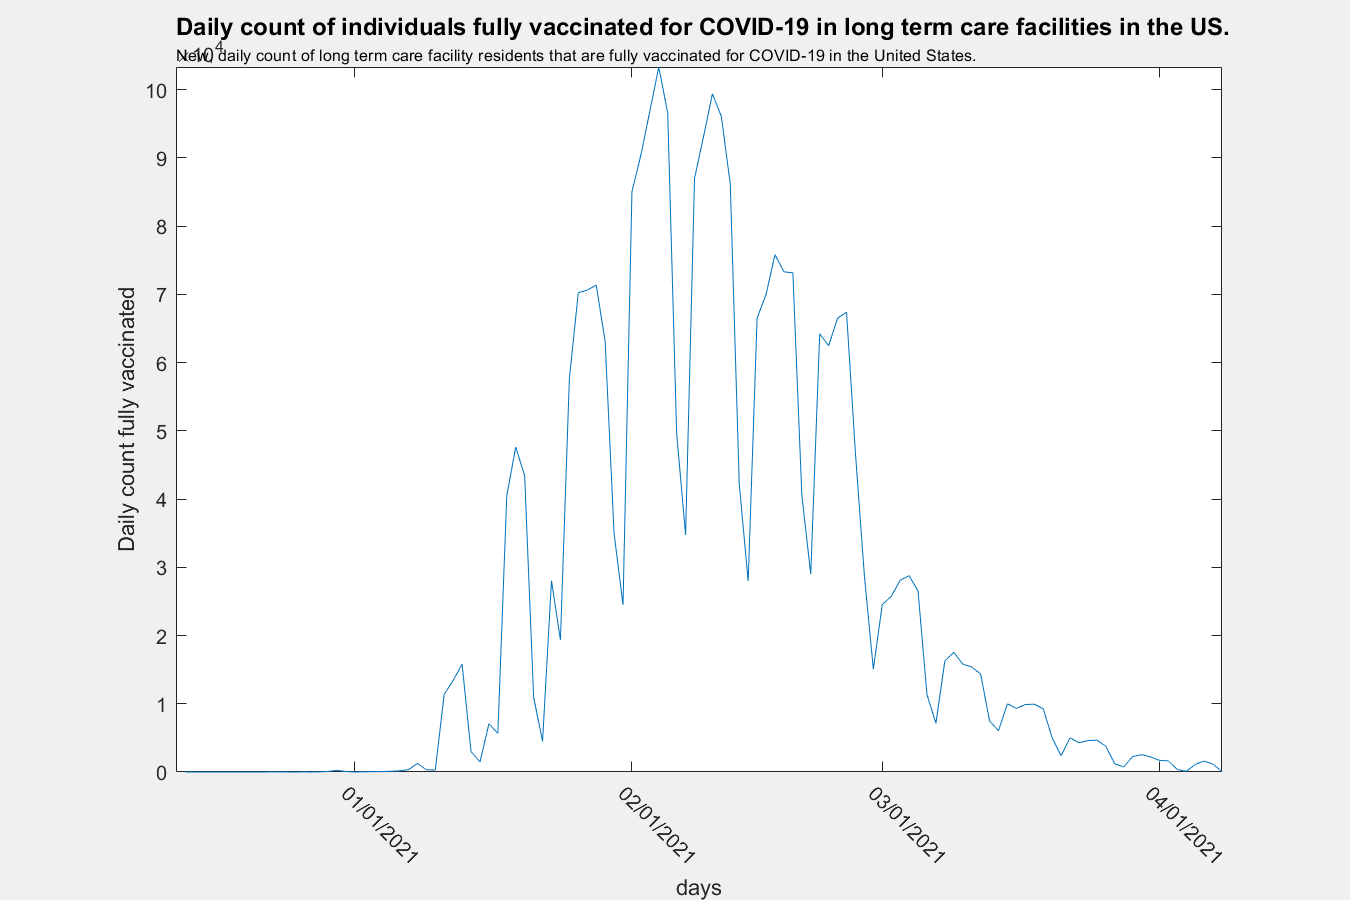
\includegraphics[width=\linewidth]{images/usa_daily_ltc_fully_vaccinated_unprocessed.png}
	\caption{Shown is the daily count for long term care residents who are fully vaccinated.}
	\label{fig:images/usa_daily_ltc_fully_vaccinated_unprocessedLabel}
\end{figure}

\begin{figure}[H]
	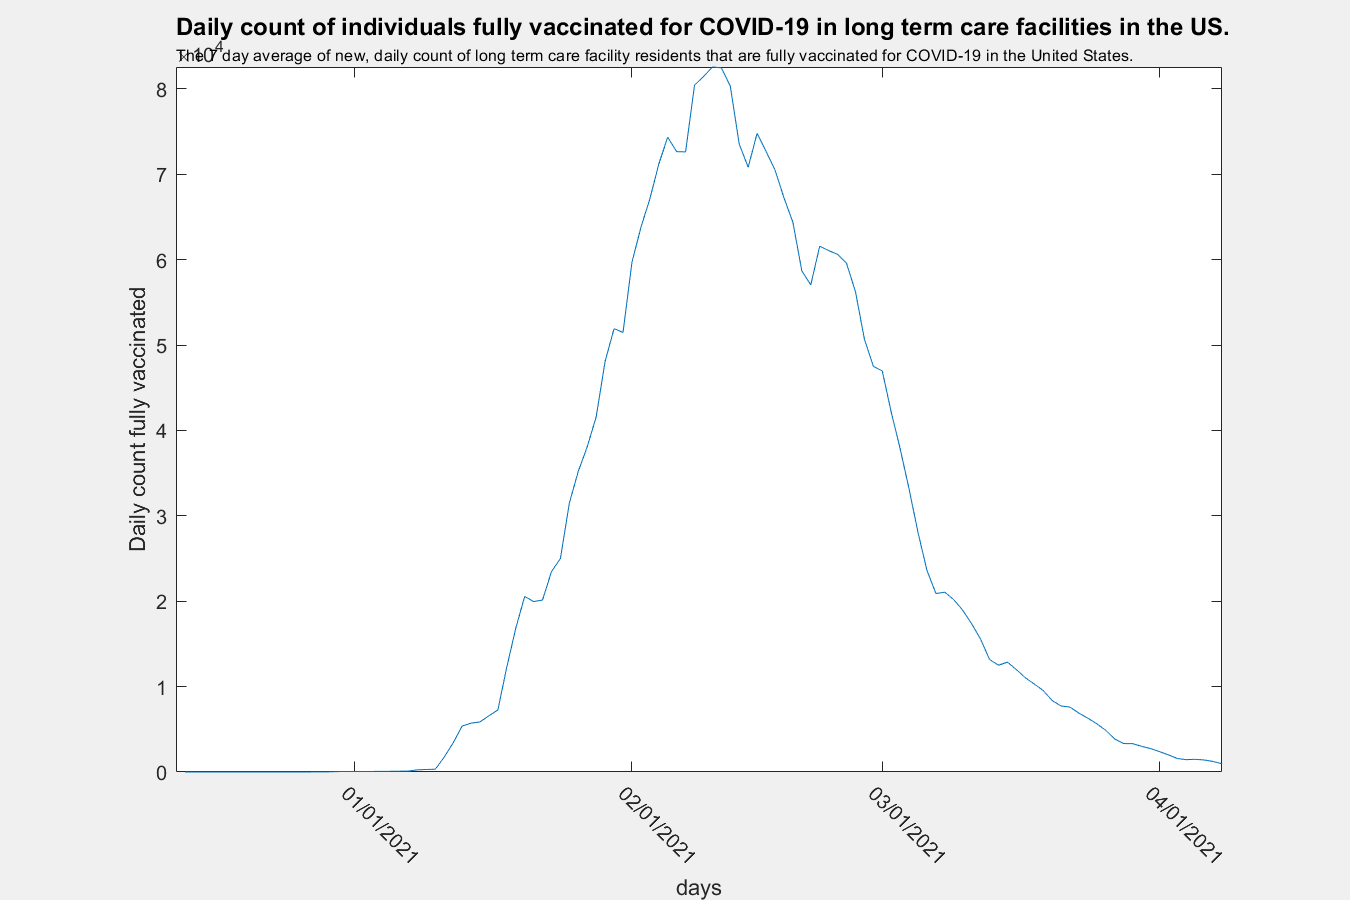
\includegraphics[width=\linewidth]{images/usa_daily_ltc_fully_vaccinated_processed.png}
	\caption{Shown is the rolling 7 day average for long term care residents who are fully vaccinated. }
	\label{fig:images/usa_daily_ltc_fully_vaccinated_processedLabel}
\end{figure}

\begin{figure}[H]
	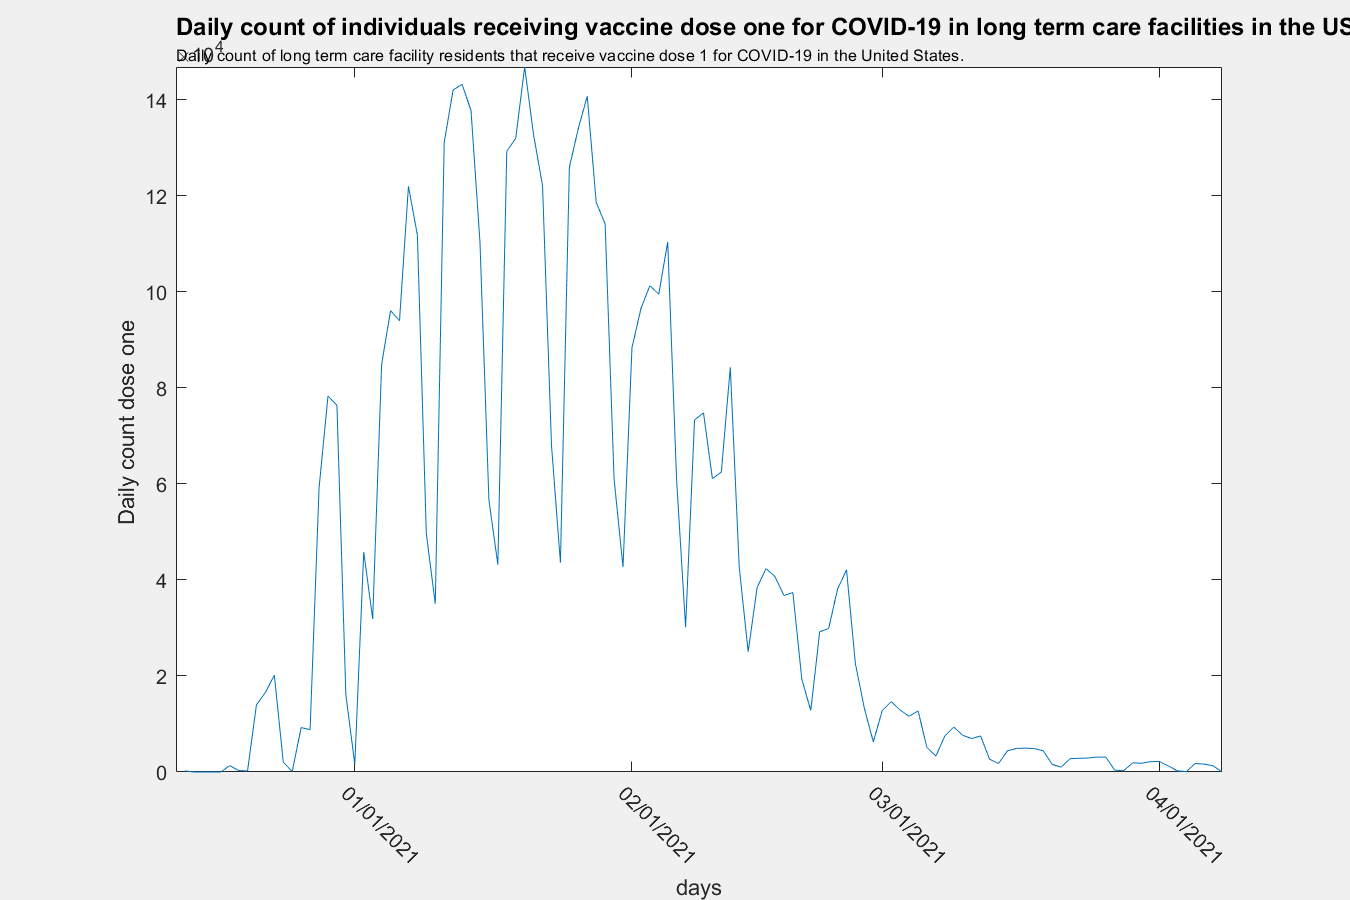
\includegraphics[width=\linewidth]{images/usa_daily_ltc_first_dose_unprocessed.png}
	\caption{}
	\label{fig:images/usa_daily_ltc_first_dose_unprocessedLabel}
\end{figure}

\begin{figure}[H]
	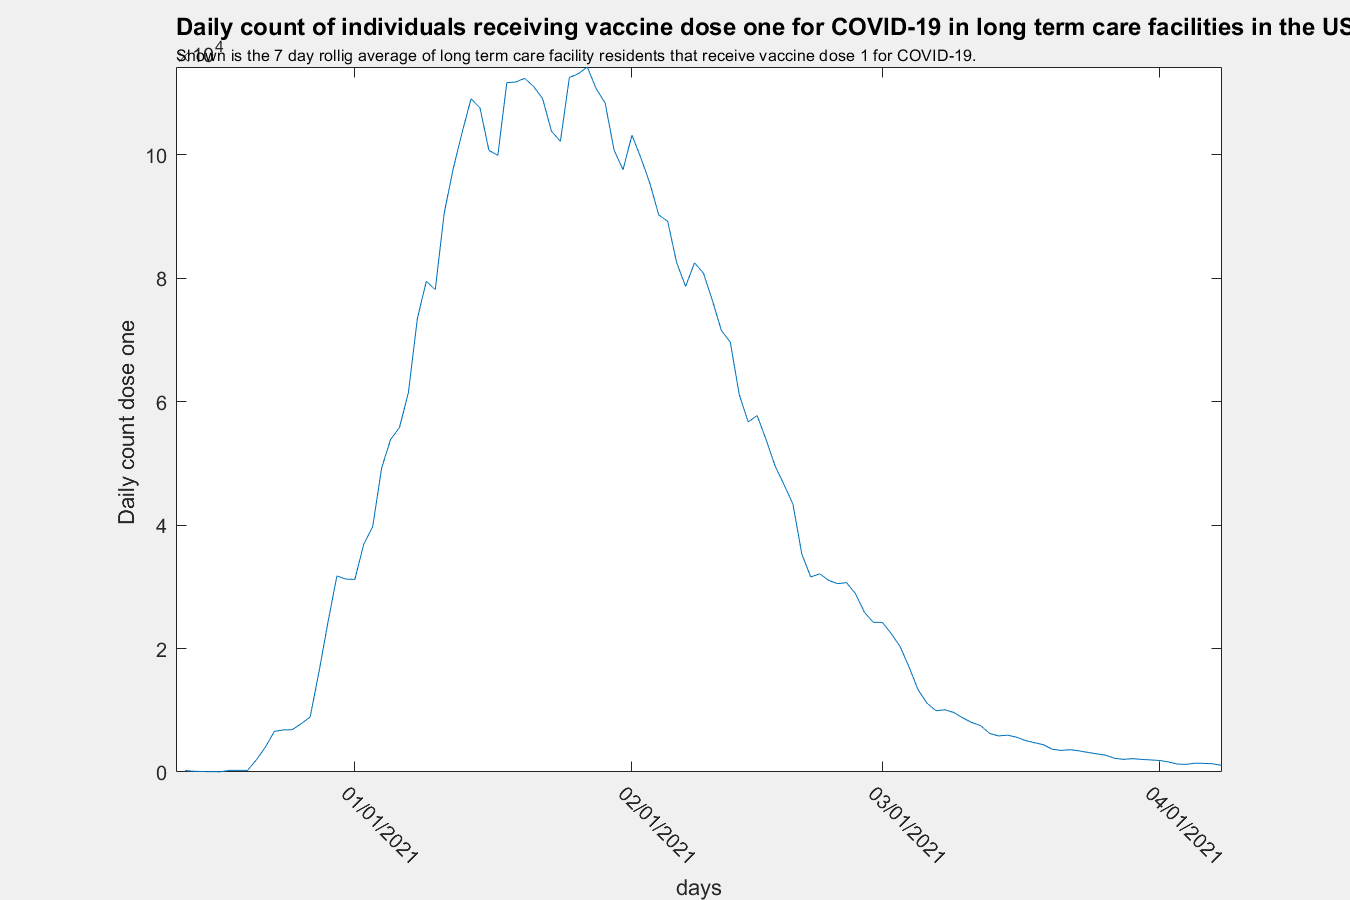
\includegraphics[width=\linewidth]{images/usa_daily_ltc_first_dose_processed.png}
	\caption{}
	\label{fig:images/usa_daily_ltc_first_dose_processedLabel}
\end{figure}

\begin{figure}[H]
	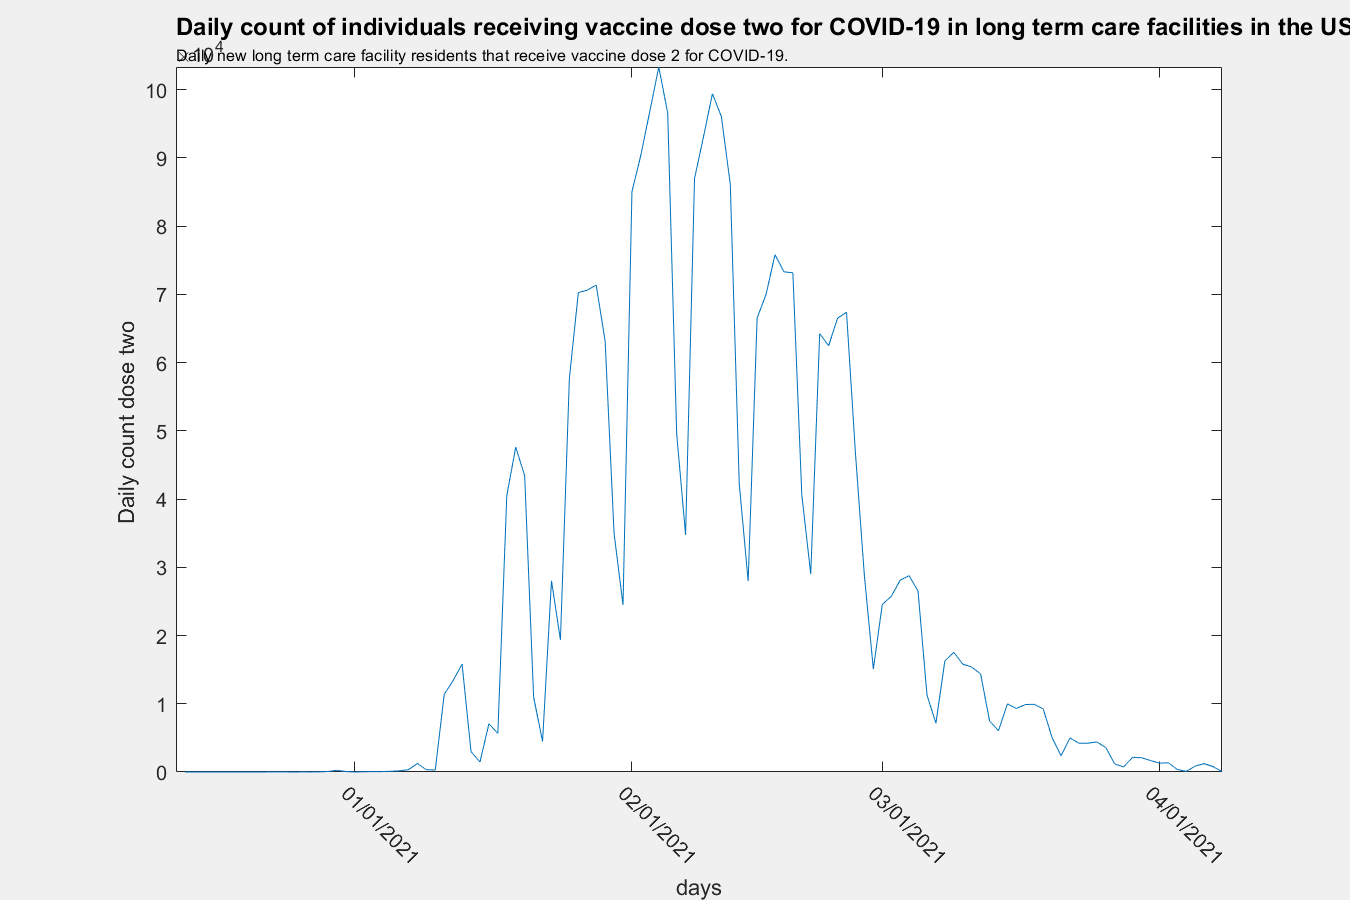
\includegraphics[width=\linewidth]{images/usa_daily_ltc_second_dose_unprocessed.png}
	\caption{}
	\label{fig:images/usa_daily_ltc_second_dose_unprocessedLabel}
\end{figure}

\begin{figure}[H]
	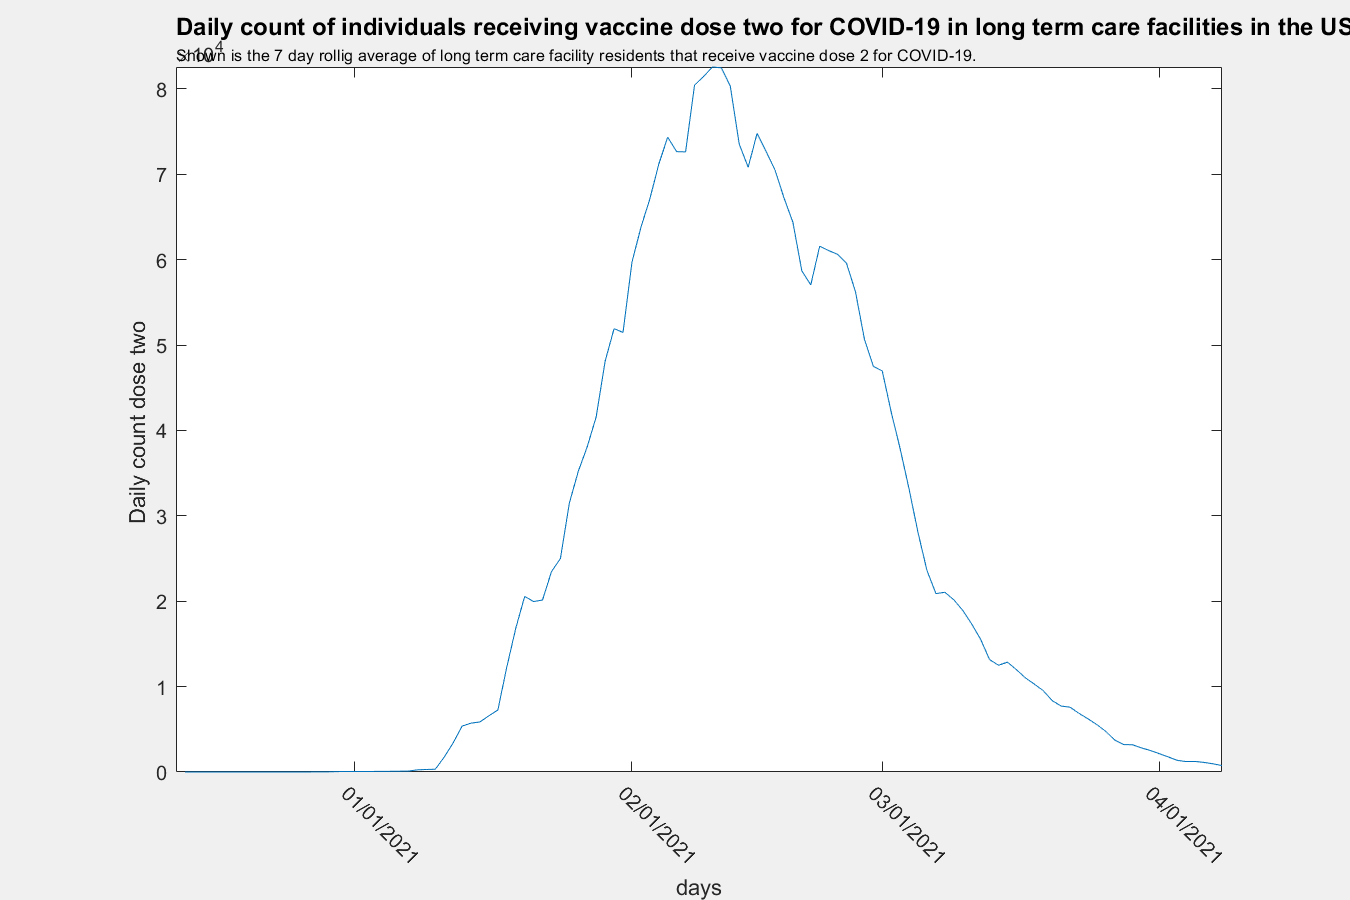
\includegraphics[width=\linewidth]{images/usa_daily_ltc_second_dose_processed.png}
	\caption{}
	\label{fig:images/usa_daily_ltc_second_dose_processedLabel}
\end{figure}

\begin{figure}[H]
	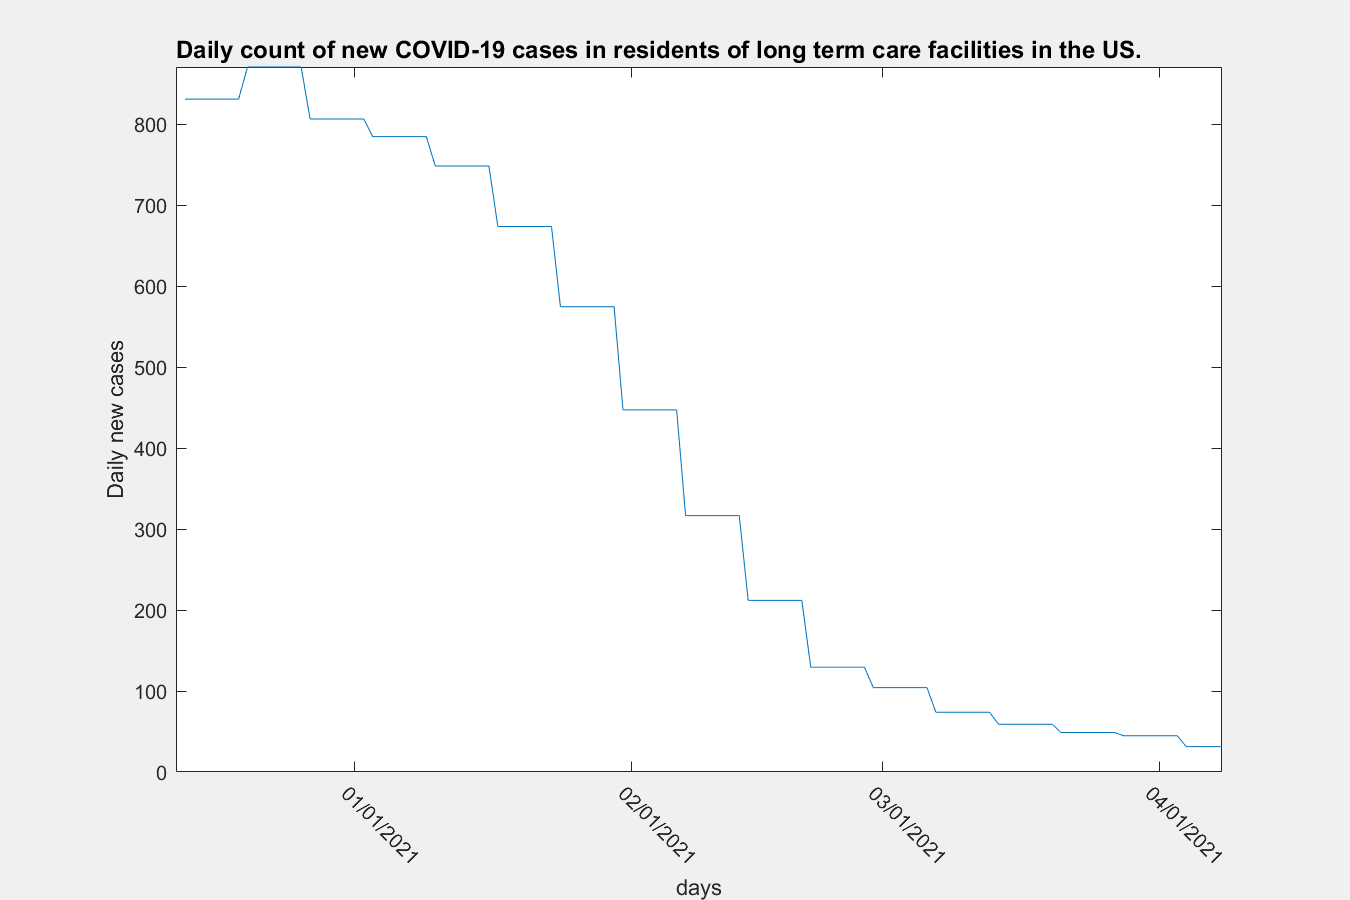
\includegraphics[width=\linewidth]{images/usa_daily_ltc_cases_unprocessed.png}
	\caption{}
	\label{fig:images/usa_daily_ltc_cases_unprocessedLabel}
\end{figure}

\subsection{Nursing Home Statistics}
\rule{\linewidth}{0.25pt}

\begin{enumerate}
	\item Histogram w/ scatterplot 
	\item Pie Chart?
	\item Graph chart for comparison?
\end{enumerate}

%------------------------------------------------

\section{Discussion}

\subsection{Model Discussion}

\begin{enumerate}
	\item Jake's model
	\item Ethan's model
\end{enumerate}


\subsection{Event Analysis Discussion}

The effectiveness of vaccinating the population against COVID-19 is undeniably positive, and is apparent through the decline in the presence of COVID-19 within the nursing home setting at the National, State, and County level. 

\vspace{5mm}

\begin{enumerate}
	\item Nationwide has declined
	\item California \& Texas have declined; Florida residents remain constant-- weird.
	\item by the time 80-90\% of first dose has been delivered, everyone is at low levels for COVID-19 in nursing home
	\item health professionals are vectors
	\item vaccinating health professionals first, and earlier saves lives faster
	\item 
	
\end{enumerate} 

%----------------------------------------------------------------------------------------
%	REFERENCE LIST
%----------------------------------------------------------------------------------------

\begin{thebibliography}{99} % Bibliography - this is intentionally simple in this template

\bibitem[Figueredo and Wolf, 2009]{Figueredo:2009dg}
Figueredo, A.~J. and Wolf, P. S.~A. (2009).
\newblock Assortative pairing and life history strategy - a cross-cultural
  study.
\newblock {\em Human Nature}, 20:317--330.
 
\end{thebibliography}

%----------------------------------------------------------------------------------------

\end{multicols}

\end{document}